%%  TESIS COMPLETA — Archivo unificado para edicion
%%  Para compilar necesitas en la misma carpeta:
%%    ThesisPUC.cls, ThesisPUC.bst, atbeginend.sty, puc.png, abrevs.tex, figs/
%%  Compilar con: pdflatex tesis_completa && bibtex tesis_completa && pdflatex tesis_completa && pdflatex tesis_completa
%% =============================================================================

\documentclass[
  msc,
  american
]{ThesisPUC_v2}

\usepackage[round, authoryear]{natbib}
\AtBeginDocument{\bibliographystyle{plainnat}}


%%%
%%% Additional Packages
%%%

  \usepackage{tabularx}
  \usepackage{multirow}
  \usepackage{multicol}
  \usepackage{colortbl}
  \usepackage[section]{placeins}
  \usepackage[%
    dvipsnames,
    svgnames,
    x11names,
    fixpdftex
  ]{xcolor}
  \usepackage{booktabs}
  \usepackage{amsmath}
  \usepackage{amssymb}
  \usepackage{enumitem}
  \usepackage{makecell}
  \usepackage{subcaption}
  \usepackage{float}
  \usepackage{tikz}
  \usetikzlibrary{shapes.geometric, arrows.meta, positioning, calc, backgrounds}
  \usepackage{graphicx}
  \graphicspath{{figs/}}


%%%
%%% Custom commands
%%%

\newcommand{\todo}[1]{\textcolor{red}{[TODO: #1]}}

\newcolumntype{L}{>{\raggedright \arraybackslash}X}
\newcolumntype{R}{>{\raggedleft \arraybackslash}X}
\newcolumntype{C}{>{\centering \arraybackslash}X}


%%%
%%% TikZ colors
%%%

\definecolor{lowlabel}{RGB}{225, 245, 238}
\definecolor{highlabel}{RGB}{250, 236, 231}
\definecolor{sslpurple}{RGB}{238, 237, 254}
\definecolor{graybox}{RGB}{241, 239, 232}
\definecolor{accentgreen}{RGB}{29, 158, 117}
\definecolor{accentorange}{RGB}{216, 90, 48}
\definecolor{pool1}{RGB}{232, 225, 247}
\definecolor{pool2}{RGB}{210, 196, 240}
\definecolor{pool3}{RGB}{182, 160, 228}
\definecolor{PUCBlue}{RGB}{0, 47, 108}
\definecolor{Accent1}{RGB}{29, 158, 117}
\definecolor{Accent2}{RGB}{216, 90, 48}


%%%
%%% TikZ macro: experimental design figure
%%%

\newcommand{\makefigone}{%
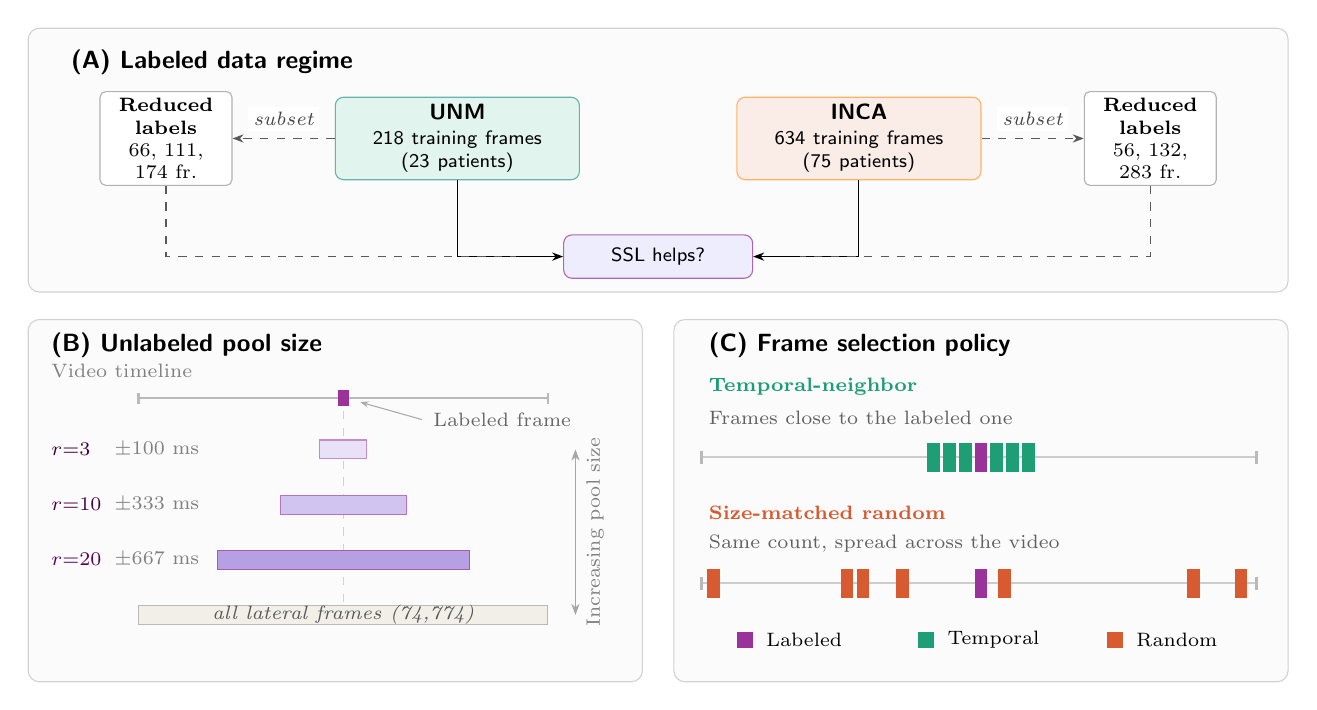
\begin{tikzpicture}[
  x=1cm, y=1cm, font=\sffamily\footnotesize,
  every node/.style={inner sep=2.5pt},
  panel/.style={draw=gray!35, rounded corners=4pt, fill=gray!3},
  box/.style={draw, rounded corners=3pt, minimum width=3.1cm, minimum height=1.0cm, text width=2.8cm, align=center},
  sslbox/.style={draw, rounded corners=3pt, fill=sslpurple, draw=violet!60, minimum width=2.4cm, minimum height=0.55cm, align=center},
  >={Stealth[length=4pt]}
]
\draw[panel] (-8.0, 0.15) rectangle (8.0, -3.20);
\draw[panel] (-8.0, -3.55) rectangle (-0.2, -8.15);
\draw[panel] ( 0.2, -3.55) rectangle ( 8.0, -8.15);
\node[font=\sffamily\small\bfseries, anchor=west] at (-7.55, -0.28) {(A) Labeled data regime};
\node[draw=gray!60, rounded corners=2pt, fill=white, align=center, font=\scriptsize, text width=1.5cm, minimum height=1.0cm] (unmsub) at (-6.25, -1.25) {\textbf{Reduced}\\\textbf{labels}\\66, 111, 174 fr.};
\node[box, fill=lowlabel, draw=teal!60] (unm) at (-2.55, -1.25) {\textbf{UNM}\\[1pt] \scriptsize 218 training frames\\[-1pt] \scriptsize (23 patients)};
\node[box, fill=highlabel, draw=orange!60] (inca) at (2.55, -1.25) {\textbf{INCA}\\[1pt] \scriptsize 634 training frames\\[-1pt] \scriptsize (75 patients)};
\node[draw=gray!60, rounded corners=2pt, fill=white, align=center, font=\scriptsize, text width=1.5cm, minimum height=1.0cm] (incasub) at (6.25, -1.25) {\textbf{Reduced}\\\textbf{labels}\\56, 132, 283 fr.};
\draw[->, dashed, thin, gray!70!black] (unm.west) -- (unmsub.east);
\draw[->, dashed, thin, gray!70!black] (inca.east) -- (incasub.west);
\node[fill=white, inner sep=2pt, font=\scriptsize\itshape, text=gray!55!black] at ($(unm.west)!0.5!(unmsub.east) + (0,0.25)$) {subset};
\node[fill=white, inner sep=2pt, font=\scriptsize\itshape, text=gray!55!black] at ($(inca.east)!0.5!(incasub.west) + (0,0.25)$) {subset};
\node[sslbox] (sslq) at (0, -2.75) {\scriptsize SSL helps?};
\coordinate (joinL) at (-1.80, -2.75); \coordinate (joinR) at ( 1.80, -2.75);
\draw[thin] (unm.south) |- (joinL); \draw[thin] (inca.south) |- (joinR);
\draw[dashed, thin, gray!70!black] (unmsub.south) |- (joinL);
\draw[dashed, thin, gray!70!black] (incasub.south) |- (joinR);
\draw[->, thin] (joinL) -- (sslq.west); \draw[->, thin] (joinR) -- (sslq.east);
\node[font=\sffamily\small\bfseries, anchor=west] at (-7.80, -3.88) {(B) Unlabeled pool size};
\draw[dashed, gray!35, very thin] (-4.00, -4.50) -- (-4.00, -7.40);
\draw[thick, gray!55] (-6.60, -4.55) -- (-1.40, -4.55);
\draw[thick, gray!55] (-6.60, -4.48) -- (-6.60, -4.62);
\draw[thick, gray!55] (-1.40, -4.48) -- (-1.40, -4.62);
\node[font=\scriptsize, gray, anchor=west] at (-7.80, -4.20) {Video timeline};
\fill[violet!80] (-4.07, -4.65) rectangle (-3.93, -4.45);
\draw[-{Stealth[length=3pt]}, gray!65, thin, shorten >=2pt] (-3.00, -4.82) -- (-3.85, -4.58);
\node[font=\scriptsize, gray!80!black, anchor=west] at (-2.95, -4.82) {Labeled frame};
\node[font=\scriptsize\bfseries, violet!45!black, anchor=west] at (-7.80, -5.20) {$r{=}3$};
\node[font=\scriptsize, gray, anchor=west] at (-7.00, -5.20) {$\pm 100$ ms};
\fill[pool1, draw=violet!45, thin] (-4.30, -5.32) rectangle (-3.70, -5.08);
\node[font=\scriptsize\bfseries, violet!55!black, anchor=west] at (-7.80, -5.90) {$r{=}10$};
\node[font=\scriptsize, gray, anchor=west] at (-7.00, -5.90) {$\pm 333$ ms};
\fill[pool2, draw=violet!55, thin] (-4.80, -6.02) rectangle (-3.20, -5.78);
\node[font=\scriptsize\bfseries, violet!70!black, anchor=west] at (-7.80, -6.60) {$r{=}20$};
\node[font=\scriptsize, gray, anchor=west] at (-7.00, -6.60) {$\pm 667$ ms};
\fill[pool3, draw=violet!65, thin] (-5.60, -6.72) rectangle (-2.40, -6.48);
\fill[graybox, draw=gray!55, thin] (-6.60, -7.42) rectangle (-1.40, -7.18);
\node[font=\scriptsize\itshape, gray!70!black] at (-4.00, -7.30) {all lateral frames (74{,}774)};
\draw[<->, gray!70, thin] (-1.05, -5.20) -- (-1.05, -7.30);
\node[font=\scriptsize, gray, rotate=90, align=center] at (-0.80, -6.25) {Increasing pool size};
\node[font=\sffamily\small\bfseries, anchor=west] at (0.55, -3.88) {(C) Frame selection policy};
\node[font=\scriptsize\bfseries, accentgreen, anchor=west] at (0.55, -4.40) {Temporal-neighbor};
\node[font=\scriptsize, gray!75!black, anchor=west] at (0.55, -4.80) {Frames close to the labeled one};
\draw[thick, gray!40] (0.55, -5.30) -- (7.60, -5.30);
\draw[thick, gray!55] (0.55, -5.22) -- (0.55, -5.38);
\draw[thick, gray!55] (7.60, -5.22) -- (7.60, -5.38);
\fill[violet!80] (4.02, -5.48) rectangle (4.18, -5.12);
\foreach \x in {3.5, 3.70, 3.90, 4.50, 4.3, 4.5, 4.7} {\fill[accentgreen] (\x-0.08, -5.48) rectangle (\x+0.08, -5.12);}
\node[font=\scriptsize\bfseries, accentorange, anchor=west] at (0.55, -6.00) {Size-matched random};
\node[font=\scriptsize, gray!75!black, anchor=west] at (0.55, -6.40) {Same count, spread across the video};
\draw[thick, gray!40] (0.55, -6.90) -- (7.60, -6.90);
\draw[thick, gray!55] (0.55, -6.82) -- (0.55, -6.98);
\draw[thick, gray!55] (7.60, -6.82) -- (7.60, -6.98);
\fill[violet!80] (4.02, -7.08) rectangle (4.18, -6.72);
\foreach \x in {0.70, 2.40, 2.60, 3.10, 4.40, 6.80, 7.40} {\fill[accentorange] (\x-0.08, -7.08) rectangle (\x+0.08, -6.72);}
\fill[violet!80] (1.00, -7.72) rectangle (1.20, -7.52); \node[font=\scriptsize, anchor=west] at (1.28, -7.62) {Labeled};
\fill[accentgreen] (3.30, -7.72) rectangle (3.50, -7.52); \node[font=\scriptsize, anchor=west] at (3.58, -7.62) {Temporal};
\fill[accentorange] (5.70, -7.72) rectangle (5.90, -7.52); \node[font=\scriptsize, anchor=west] at (5.98, -7.62) {Random};
\end{tikzpicture}%
}


%%%
%%% Misc.
%%%

\usecolour{true}


%%%
%%% Metadata
%%%

\author{Sebastian Quispe Arias}
\authorR{Quispe Arias, Sebastian}

\advisor{Paulo Ivson Netto Santos}{Prof.}
\advisorR{Ivson Netto Santos, Paulo}

\coadvisor{Luiz Fernando Trindade Santos}{Dr.}
\coadvisorR{Trindade Santos, Luiz Fernando}

\title{Aprendizado semi-supervisionado para segmenta\c{c}\~{a}o de
  v\'{e}rtebras cervicais em estudos de videofluoroscopia da
  degluti\c{c}\~{a}o}

\titleuk{Semi-supervised learning for cervical vertebra segmentation
  in videofluoroscopic swallowing studies}

\day{24}
\month{September}
\year{2026}

\city{Rio de Janeiro}
\CDD{004}
\department{Inform\'{a}tica}
\program{Inform\'{a}tica}
\school{Centro T\'{e}cnico Cient\'{i}fico}
\university{Pontif\'{i}cia Universidade Cat\'{o}lica do Rio de Janeiro}
\uni{PUC-Rio}


%%%
%%% Jury
%%%

\jury{%
  \jurymember{Alberto Barbosa Raposo}{Prof.}
    {Departamento de Inform\'{a}tica}{PUC-Rio}
  \jurymember{Geraldo Braz J\'{u}nior}{Prof.}
    {}{UFMA}
  \jurymember{Cesar Augusto Sierra Franco}{Dr.}
    {Tecgraf}{PUC-Rio}
}


%%%
%%% Resume
%%%

\resume{%
  Graduated in Industrial Engineering from Pontificia Universidad Cat\'{o}lica del Per\'{u} (PUCP).
  Worked as a research fellow in data science at ZANE.
  Started the M.Sc. program in Informatics at PUC-Rio in the second semester of 2024, under the supervision of Prof. Paulo Ivson Netto Santos.
  Research interests include computer vision, deep learning, and medical image analysis.}


%%%
%%% Acknowledgment
%%%

\acknowledgment{%
  \noindent I would like to express my gratitude to those who made this work possible.
  \bigskip

  \noindent To my advisor, Prof. Paulo Ivson Netto Santos, for his guidance and support during my master's studies.
  \bigskip

  \noindent To Luiz Fernando Santos, for the many conversations and for guiding me through this work.
  \bigskip

  \noindent To my family, for their support all this time.
  \bigskip

  \noindent This study was financed in part by the Coordena\c{c}\~{a}o de Aperfei\c{c}oamento de Pessoal de N\'{i}vel Superior -- Brasil (CAPES) -- Finance Code 001.
}


%%%
%%% Catalog prekeywords
%%%

\catalogprekeywords{%
  \catalogprekey{Inform\'{a}tica}%
}


%%%
%%% Keywords
%%%

\keywords{%
  \key{Videofluoroscopia}
  \key{Segmenta\c{c}\~{a}o de V\'{e}rtebras Cervicais}
  \key{Aprendizado Semi-supervisionado}
  \key{Pseudo-rotulagem}
  \key{Mean Teacher}
  \key{Aprendizado Profundo}
}

\keywordsuk{%
  \key{Videofluoroscopy}%
  \key{Cervical Vertebra Segmentation}%
  \key{Semi-supervised Learning}%
  \key{Pseudo-labeling}%
  \key{Mean Teacher}%
  \key{Deep Learning}
}


%%%
%%% Front matter headings
%%%

\abreviationstitleuk{List of Abbreviations}


%%%
%%% Abstract (Portuguese)
%%%

\abstract{%
  Em estudos videofluorosc\'{o}picos da degluti\c{c}\~{a}o (VFSS), as
  v\'{e}rtebras cervicais servem como refer\^{e}ncias anat\^{o}micas para a
  medi\c{c}\~{a}o objetiva da cinem\'{a}tica da degluti\c{c}\~{a}o, mas a anota\c{c}\~{a}o ao
  n\'{i}vel do pixel \'{e} custosa e raramente est\'{a} dispon\'{i}vel em larga
  escala. O aprendizado semi-supervisionado (SSL) pode explorar
  quadros n\~{a}o rotulados naturalmente presentes nos v\'{i}deos de VFSS,
  mas seu papel nesta tarefa de segmenta\c{c}\~{a}o permanece pouco
  estudado. Esta disserta\c{c}\~{a}o avalia sistematicamente o SSL para a
  segmenta\c{c}\~{a}o de v\'{e}rtebras cervicais usando pseudo-rotulagem e
  Mean Teacher em dois conjuntos de dados institucionais: o
  subconjunto da University of New Mexico (UNM) do TalkBank com 218
  quadros de treinamento, e o subconjunto do Instituto Nacional de
  C\^{a}ncer (INCA) com 634 quadros de treinamento, totalizando 342
  execu\c{c}\~{o}es de treinamento. Em todos os or\c{c}amentos de r\'{o}tulos
  testados em ambos os conjuntos de dados, o SSL alcan\c{c}ou F1
  compar\'{a}vel ou superior ao treinamento supervisionado, com o Mean
  Teacher preservando a qualidade da segmenta\c{c}\~{a}o sob redu\c{c}\~{a}o
  agressiva de r\'{o}tulos. Os maiores ganhos do SSL ocorreram onde a
  linha de base supervisionada ainda n\~{a}o havia saturado: no UNM, o
  Mean Teacher alcan\c{c}ou F1~=~0.860 versus F1~=~0.801 do
  supervisionado. No INCA, o SSL n\~{a}o produziu
  melhoria em 25\% dos r\'{o}tulos ou mais; com apenas 10\% dos
  r\'{o}tulos, o Mean Teacher alcan\c{c}ou F1~=~0.865 sobre F1~=~0.844.
  Esses resultados indicam que o SSL pode
  ser praticamente \'{u}til em cen\'{a}rios de VFSS com poucos r\'{o}tulos, ao
  explorar quadros n\~{a}o rotulados j\'{a} presentes nos v\'{i}deos.}


%%%
%%% Abstract (English)
%%%

\abstractuk{%
  In videofluoroscopic swallowing studies (VFSS), cervical
  vertebrae serve as anatomical references for objective
  measurement of swallowing kinematics, but pixel-level annotation
  is costly and rarely available at scale. Semi-supervised
  learning (SSL) can exploit unlabeled frames naturally present in
  VFSS video, but its role in this segmentation task remains
  underexplored. This thesis systematically evaluates SSL for
  cervical vertebra segmentation using pseudo-labeling and Mean
  Teacher on two institutional datasets: the University of New
  Mexico (UNM) TalkBank subset with 218 training frames, and the
  Instituto Nacional de C\^ancer (INCA) subset with 634 training
  frames, totaling 342 training runs. Across all tested label
  budgets in both datasets, SSL achieved F1 comparable to or above
  supervised training, with Mean Teacher preserving segmentation
  quality under aggressive label reduction. The
  largest SSL gains occurred where the supervised baseline had not
  yet saturated: in UNM, Mean Teacher reached F1~=~0.860 vs
  supervised F1~=~0.801. In INCA, SSL
  produced no improvement at 25\% labels and above; with only 10\%
  labels, Mean Teacher reached F1~=~0.865 over F1~=~0.844.
  These results indicate that SSL can be
  practically useful in low-label VFSS settings by exploiting
  unlabeled frames already present in the videos.}


%%%
%%% Dedication
%%%

\dedication{%
  To my family, for their support\\
and encouragement.
}


%%%
%%% Epigraph (NOT USED - commented out to suppress rendering)
%%%

% \epigraph{%
%   TODO: Your epigraph here.
% }
% \epigraphauthor{TODO: Author}
% \epigraphbook{TODO: Source}


%%%
%%% Hyphenation
%%%

\hyphenation{vi-deo-fluo-ros-co-py vi-deo-fluo-ros-co-pic}


%% =============================================================================
%%  DOCUMENT
%% =============================================================================

\begin{document}


%% =============================================================================
%%  CHAPTER 1 — Introduction
%% =============================================================================

\chapter{Introduction}
\label{chap:intro}

\section{Dysphagia and the videofluoroscopic swallowing study}
\label{sec:intro-background}

Dysphagia, the medical term for swallowing impairment, is a prevalent condition that compromises both nutrition and airway protection across diverse patient populations~\citep{ref_logemann}. It is particularly frequent in patients treated for head and neck cancer, where surgery, radiotherapy, and chemotherapy can disrupt the anatomical and neuromuscular structures involved in swallowing. Beyond reducing quality of life, dysphagia carries serious clinical consequences: silent aspiration of food or liquid into the airway can lead to aspiration pneumonia, malnutrition, dehydration, and increased mortality. A central diagnostic challenge is that aspiration can occur silently, without triggering a protective cough reflex, and therefore cannot be reliably detected by external observation alone~\citep{ref_smith1999_silent}.

The videofluoroscopic swallowing study (VFSS) is the most widely used instrumental examination for evaluating dysphagia. During a VFSS, continuous lateral X-ray images are recorded while the patient swallows a radio-opaque (barium) contrast bolus, producing a dynamic visualization of the oral, pharyngeal, and esophageal phases of swallowing~\citep{ref_kendall2000}. This in-vivo, dynamic view allows direct observation of events that cannot be inferred from external examination, including silent aspiration, bolus residue, and abnormal timing of pharyngeal constriction~\citep{ref_shu_review}.

Beyond qualitative inspection, VFSS images also support quantitative analyses of swallowing kinematics. These analyses rely on the cervical vertebrae C2--C4 as a consistent anatomical reference for normalization of kinematic measurements via the C2--C4 anatomical scalar~\citep{ref_molfenter,ref_steele_norms}, for defining coordinate systems for hyoid bone tracking~\citep{ref_kim2021}, and for region-of-interest definition in airway-invasion analysis~\citep{ref_lee2020}.

The literature distinguishes two computational approaches for analyzing C2--C4 in VFSS images: landmark-based methods, which predict the corner coordinates of each vertebra~\citep{ref_zhang2021,ref_li2024}, and segmentation-based methods, which predict a pixel-level mask covering the vertebral region~\citep{ref_lee2020,ref_kim2021}. The choice between them depends on the downstream task: landmark coordinates are sufficient for the anatomical scalar and for measurements based on specific reference points, while pixel-level masks become necessary when the full spatial extent of the vertebral region is needed, such as for dynamic regions of interest that follow head motion~\citep{ref_lee2020}, or for analyses that require the vertebral shape rather than isolated reference points~\citep{ref_mekata2013,ref_fujinaka}.

This thesis focuses on the segmentation approach, motivated by those downstream tasks that require pixel-level masks rather than only landmark coordinates. Figure~\ref{fig:vfss-example} illustrates the segmentation target. However, obtaining pixel-level vertebral masks at scale requires substantial manual annotation effort, an annotation bottleneck that the next section addresses.

\begin{figure}[!htbp]
  \centering
  \includegraphics[width=\textwidth]{vfss_example.pdf}
  \caption[Example VFSS frame with manual C2--C4 segmentation.]{Example VFSS frame. Left: original grayscale lateral frame as acquired by the videofluoroscopic system. Right: same frame with the manual C2--C4 segmentation mask overlaid in green.}
  \label{fig:vfss-example}
\end{figure}


\section{Annotation of cervical vertebrae in VFSS}
\label{sec:intro-bottleneck}

Segmenting the C2--C4 cervical vertebral region in VFSS is technically challenging for several reasons inherent to the imaging modality. The dynamic fluoroscopic acquisition produces images that are noisier and grainier due to the low radiation dose used to limit patient exposure, compared to static radiographs. The ingested barium contrast can also locally obscure bony boundaries during bolus transit. In addition, the vertebrae project onto a two-dimensional image alongside overlapping soft-tissue and bony structures (mandible, hyoid, skull base), making the boundaries of C2--C4 visually ambiguous in many frames. These factors prevent simple intensity-based segmentation and motivate the use of learning-based approaches.

The annotated data needed to train such models is costly to obtain in this domain. Producing pixel-level annotations of the cervical vertebrae in VFSS requires task-specific anatomical knowledge, because annotators must distinguish vertebral boundaries from overlapping structures and handle frames where the bony contours are partially obscured, with each frame typically taking 2--3 minutes of focused annotation work. Even among trained annotators, the boundaries of C2--C4 are not always unambiguously defined, resulting in non-negligible inter-rater variability. Combined with privacy constraints and ethical regulations that restrict the sharing of clinical data, these factors keep publicly accessible VFSS datasets with pixel-level annotations scarce~\citep{ref_fakhry2025,ref_sanjeevi2025}.

Despite these constraints, the same VFSS recordings contain far more unlabeled frames. Each lateral VFSS video provides a continuous sequence of frames, of which only a small fraction is typically selected for annotation; the rest remain accessible to the research team but unused under a fully supervised training paradigm. This labeled--unlabeled imbalance is summarized in Figure~\ref{fig:annotation-bottleneck}, and suggests training strategies that can exploit both sources of data jointly.

\begin{figure}[!htbp]
  \centering
  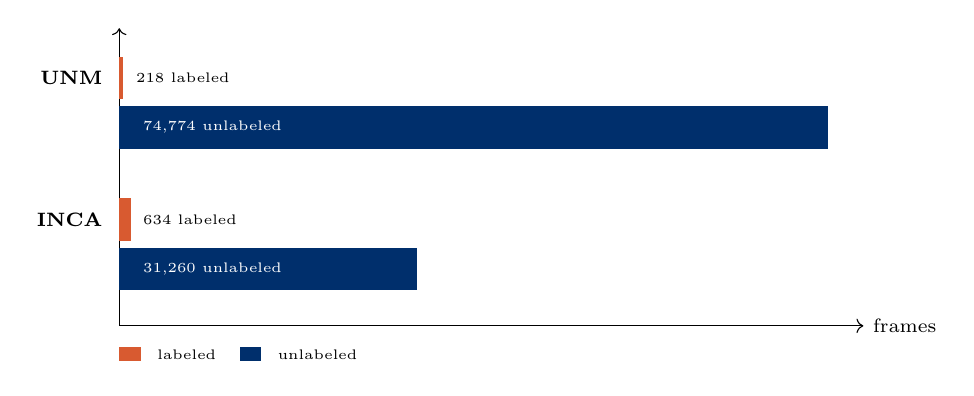
\begin{tikzpicture}[scale=0.9]
    % Eje
    \draw[->] (0,0) -- (10.5,0) node[right] {\scriptsize frames};
    \draw[->] (0,0) -- (0,4.2);

    % UNM
    \node[anchor=east] at (-0.1,3.5) {\scriptsize \textbf{UNM}};
    \fill[Accent2] (0,3.2) rectangle (0.05,3.8);
    \node[anchor=west, font=\tiny] at (0.1,3.5) {218 labeled};
    \fill[PUCBlue] (0,2.5) rectangle (10,3.1);
    \node[anchor=west, font=\tiny, white] at (0.2,2.8) {74{,}774 unlabeled};

    % INCA
    \node[anchor=east] at (-0.1,1.5) {\scriptsize \textbf{INCA}};
    \fill[Accent2] (0,1.2) rectangle (0.16,1.8);
    \node[anchor=west, font=\tiny] at (0.2,1.5) {634 labeled};
    \fill[PUCBlue] (0,0.5) rectangle (4.2,1.1);
    \node[anchor=west, font=\tiny, white] at (0.2,0.8) {31{,}260 unlabeled};

    % Leyenda
    \fill[Accent2] (0,-0.5) rectangle (0.3,-0.3);
    \node[anchor=west, font=\tiny] at (0.4,-0.4) {labeled};
    \fill[PUCBlue] (1.7,-0.5) rectangle (2,-0.3);
    \node[anchor=west, font=\tiny] at (2.1,-0.4) {unlabeled};
  \end{tikzpicture}
  \caption[Labeled and unlabeled training frames in UNM and INCA.]{Labeled and unlabeled training frames in the two VFSS datasets used in this thesis. Pixel-level annotations are scarce relative to the much larger pool of unlabeled frames available from the same recordings (ratios approximately 343:1 in UNM and 49:1 in INCA).}
  \label{fig:annotation-bottleneck}
\end{figure}


\section{Semi-supervised learning for VFSS segmentation}
\label{sec:intro-ssl}

Semi-supervised learning (SSL) is a class of training methods that addresses this kind of asymmetry by jointly using a small labeled subset and a larger pool of unlabeled examples during training. In this way, unlabeled frames that would otherwise be discarded under fully supervised training can still contribute during training. Figure~\ref{fig:ssl-overview} summarizes this setup for the segmentation task.

\begin{figure}[!htbp]
  \centering
  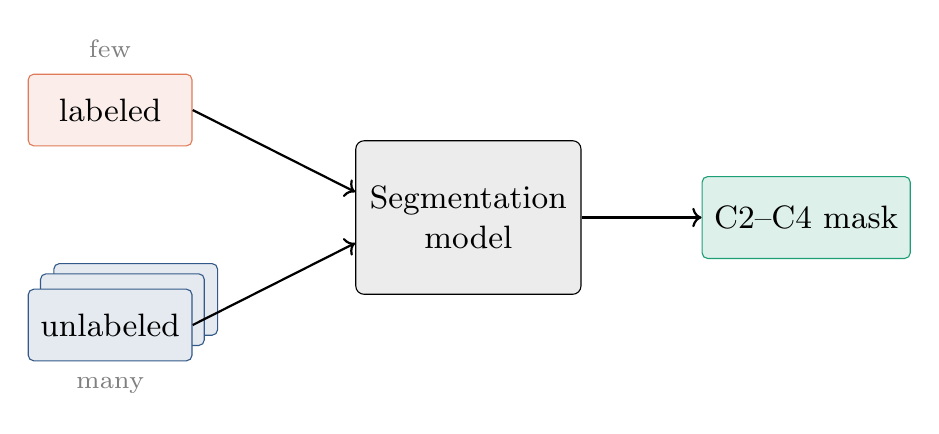
\begin{tikzpicture}[
    scale=1.3, transform shape,
    labeledbox/.style={draw=Accent2!80, fill=Accent2!10, rounded corners=2pt, minimum width=1.6cm, minimum height=0.7cm, font=\small},
    unlabeledbox/.style={draw=PUCBlue!80, fill=PUCBlue!10, rounded corners=2pt, minimum width=1.6cm, minimum height=0.7cm, font=\small},
    model/.style={draw=black, fill=gray!15, rounded corners=3pt, minimum width=2.2cm, minimum height=1.5cm, font=\small, align=center}
  ]
    % Labeled (arriba izq)
    \node[labeledbox] (l1) at (0, 1.3) {labeled};
    \node[font=\scriptsize, gray, above=1pt of l1] {few};

    % Unlabeled stack (abajo izq)
    \node[unlabeledbox] (u3) at (0.25, -0.55) {};
    \node[unlabeledbox] (u2) at (0.12, -0.65) {};
    \node[unlabeledbox] (u1) at (0, -0.8) {unlabeled};
    \node[font=\scriptsize, gray, below=1pt of u1] {many};

    % Model (centro)
    \node[model] (m) at (3.5, 0.25) {Segmentation\\ model};

    % Output (derecha)
    \node[draw=Accent1, fill=Accent1!15, rounded corners=2pt, minimum width=2cm, minimum height=0.8cm, font=\small] (mask) at (6.8, 0.25) {C2--C4 mask};

    % Flechas
    \draw[->, thick] (l1.east) -- ([yshift=0.25cm]m.west);
    \draw[->, thick] (u1.east) -- ([yshift=-0.25cm]m.west);
    \draw[->, thick] (m.east) -- (mask.west);
  \end{tikzpicture}
  \caption[Semi-supervised learning overview.]{Semi-supervised learning overview. A segmentation model is trained jointly on a small set of labeled frames and a larger pool of unlabeled frames drawn from the same VFSS recordings, and outputs a pixel-level C2--C4 mask at inference.}
  \label{fig:ssl-overview}
\end{figure}

This setting matches the structure of VFSS data. Each video provides a small set of annotated frames and a much larger number of unlabeled ones, all drawn from the same VFSS recordings as the annotated ones. Because the frames within a video form a continuous swallowing sequence, those close to an annotated frame in time tend to be visually similar, while more distant frames may depict different phases of the swallow. The combination of abundant unlabeled data and this temporal structure makes VFSS a setting where both the amount and the selection of unlabeled frames may matter.

Despite this natural fit, classical SSL has not been systematically applied to VFSS segmentation. Recent work in VFSS has explored other paradigms for reducing annotation burden, including active learning with expert-in-the-loop corrections~\citep{ref_cubero2025}, test-time training on foundation models~\citep{ref_zeng_ttt}, and weakly supervised, self-supervised, or unsupervised approaches applied to other VFSS segmentation targets. In adjacent fluoroscopic domains, classical teacher-student SSL has shown promise for vessel segmentation in X-ray angiography video~\citep{ref_luo_smart2026}. To the best of our knowledge, however, the joint use of labeled and unlabeled frames drawn from the same VFSS recordings has not been examined for VFSS segmentation.


\section{Research questions}
\label{sec:intro-rqs}

Applying classical SSL to vertebra segmentation in VFSS raises three practical questions that have not been addressed jointly in prior work.

\textbf{RQ1.} Under what labeled-data regime does classical SSL improve vertebra segmentation in VFSS? The benefit of SSL is known to depend on the amount of available annotation, but this regime has not been characterized for VFSS.

\textbf{RQ2.} How does the size of the unlabeled pool affect SSL performance in this setting? General SSL research has shown that not all unlabeled examples contribute equally~\citep{ref_ren2020} and that performance can degrade with out-of-distribution unlabeled data~\citep{ref_oliver2018}; the appropriate pool size for VFSS video remains an open question.

\textbf{RQ3.} Given this temporal structure, does temporal-neighbor frame selection provide an advantage over size-matched random selection, or do both yield comparable performance?

Although related questions have been examined in other medical imaging contexts~\citep{ref_fu2019}, their joint study in classical SSL for VFSS segmentation has yet to be addressed.


\section{Contributions}
\label{sec:intro-contribs}

The contributions of this thesis are:

\begin{itemize}
\renewcommand{\labelitemi}{--}
\item \textbf{A systematic evaluation of semi-supervised learning} for cervical vertebra segmentation in VFSS, using pseudo-labeling and Mean Teacher across two institutional datasets, showing that SSL achieves Dice scores comparable to or above supervised training at matched label budgets, with the clearest gains when supervised performance has not yet saturated.

\item \textbf{A characterization of how SSL performance changes} across different labeled-data budgets and how it interacts with the unlabeled pool size and the frame selection policy in this domain.

\item \textbf{A comparison of the SSL results against six supervised architectures}, including a Kim-inspired BiFPN-U-Net adapted from the VFSS literature, with nnU-Net included as a self-configuring reference.
\end{itemize}

Rather than proposing a new SSL algorithm, this thesis empirically characterizes how classical SSL behaves in a domain where it has not previously been examined, and may inform similar studies in other VFSS segmentation targets and related fluoroscopic imaging tasks.

The remainder of this thesis is organized as follows. Chapter~2 reviews related work in VFSS analysis and semi-supervised medical image segmentation. Chapter~3 describes the datasets, architecture, SSL methods, and unlabeled pool construction. Chapter~4 presents the results and discusses limitations. Chapter~5 concludes and outlines future work.


%% =============================================================================
%%  CHAPTER 2 — Related work
%% =============================================================================

\chapter{Related work}
\label{chap:related}

\section{Cervical vertebra analysis in VFSS}
\label{sec:related-vertebra}

Automated analysis of cervical vertebrae in VFSS has been approached mainly through landmark localization and semantic segmentation. \citet{ref_zhang2021} trained a two-stage CNN to localize C2--C4 corner landmarks, reporting a mean localization distance of 4.20~px on an independent test set of 70 healthy subjects. \citet{ref_li2024} used a Full-HRNet for simultaneous detection of the hyoid bone and C2--C4 corners, reaching 2.38~px mean error. \citet{ref_cubero2025} localized ten regions of interest via an iterative nnU-Net with expert-in-the-loop corrections (1.6~px mean error on a healthy cohort). None of these approaches produces pixel-level masks of the cervical vertebral region as the primary target, which limits their use in downstream tasks requiring the full spatial extent of the vertebrae.

On the segmentation side, \citet{ref_fujinaka} segmented cervical intervertebral \emph{disks} (rather than the vertebral bodies) with a patch-based CNN (F-measure 0.593). \citet{ref_lee2020} segmented the cervical spinal column as a preprocessing step to define a dynamic region of interest for airway-invasion detection. \citet{ref_kim2021} used a BiFPN-U-Net(T) to segment hyoid, spine, and a reference coin for hyoid tracking (Dice 90.9\% across three classes).

In these works the spine is an auxiliary structure rather than the segmentation target. In concurrent work, two foundation-model approaches address vertebrae directly as a segmentation target: \citet{ref_zeng_ttt} apply test-time training on MedSAM to segment individual C1--C7 vertebrae among 12 anatomies (average Dice 0.868), with full annotations on a source domain and manual point prompts at test time; \citet{ref_zeng_distill2025} distill knowledge from multiple vision foundation models (MedSAM, RAD-DINO, MedCLIP) into a lightweight student for the same 12 anatomies, but training itself relies on annotated reference masks. None of these works uses classical SSL or studies how pool size and selection policy affect performance.

\section{Alternatives to full supervision in VFSS}
\label{sec:related-alternatives}

Several recent VFSS studies have explored alternatives to full supervision, with the works most relevant to ours focusing on bolus or pharyngeal-phase analysis. \citet{ref_bandini2022} demonstrated weakly-supervised bolus localization and pharyngeal-phase detection using class activation maps, requiring only the initial and final frames of the pharyngeal phase as annotation, though their approach does not incorporate unlabeled data during training. \citet{ref_martinovic2025} used self-supervised pre-training (contrastive random walk) to learn representations from unlabeled VFSS frames, but their downstream bolus segmentation is fully supervised, with unlabeled data used only in the pretext task. An unsupervised convolutional autoencoder for bolus and residue segmentation~\citep{ref_unsup_bolus2025} operates without any pixel-level annotations, achieving an intersection-over-union of 61\% for bolus, but this lies at the opposite end of the supervision spectrum from SSL. These works reflect interest in reducing annotation dependence in VFSS, but the classical SSL setting (joint training on labeled and unlabeled data) remains underexplored.

\section{Semi-supervised medical image segmentation}
\label{sec:related-ssl}

SSL for medical image segmentation has been studied through several method families. Three widely used methods are teacher--student frameworks~\citep{ref_mean_teacher}, pseudo-labeling~\citep{ref_fixmatch}, and cross-pseudo supervision~\citep{ref_cps}. These methods have been applied across multiple organs~\citep{ref_ssl_survey,ref_han2024}, but not to VFSS segmentation.

A separate line of work has examined how the composition of the unlabeled pool affects SSL performance. \citet{ref_ren2020} showed that not all unlabeled examples contribute equally to SSL outcomes. \citet{ref_oliver2018} demonstrated that performance can degrade when unlabeled data are out-of-distribution with respect to the labeled set. More recent work on data selection~\citep{ref_rdss2024} further shows that the choice of which examples to include affects SSL results. However, these three studies examined image classification with i.i.d.\ data. Their conclusions do not necessarily transfer to segmentation in medical video, where neighboring frames are temporally related.

In adjacent fluoroscopic domains, \citet{ref_luo_smart2026} recently proposed SMART, a SAM3-based teacher--student framework with motion-aware consistency and progressive confidence regularization for coronary vessel segmentation in X-ray angiography video, achieving over six percentage points of Dice improvement with only 16 labeled videos. Their work shows that teacher--student SSL can be effective in X-ray angiography video, but it does not study pool size or selection policy in VFSS segmentation. \citet{ref_fu2019} investigated the trade-off between labeled and unlabeled data quantity for Mean Teacher in laparoscopic liver segmentation, finding that more unlabeled data does not always improve performance. These findings motivate evaluating SSL across different labeled-data regimes rather than at a single annotation budget. Their study varied only the quantity of unlabeled frames using random selection and did not compare different selection strategies or examine the effect of temporal proximity. This thesis examines both dimensions in VFSS video, varying the unlabeled pool size and the frame selection policy.


%% =============================================================================
%%  CHAPTER 3 — Methodology
%% =============================================================================

\chapter{Methodology}
\label{chap:method}

\section{Problem formulation}
\label{sec:method-formulation}

The task addressed in this work is the pixel-level binary segmentation of the C2--C4 cervical vertebral region in VFSS frames. Each dataset is partitioned into a labeled subset $\mathcal{L} = \{(x_i, y_i)\}_{i=1}^{N_L}$, where $x_i$ is a VFSS frame and $y_i$ is its corresponding binary mask, and an unlabeled subset $\mathcal{U} = \{x_j\}_{j=1}^{N_U}$, with $N_U \gg N_L$ given the abundance of unlabeled VFSS frames. A segmentation model $f_\theta$ is trained jointly on $\mathcal{L}$ and $\mathcal{U}$ using SSL methods that use the unlabeled frames to complement the limited labeled supervision. The study evaluates how this joint training depends on the size of $\mathcal{L}$, the size of $\mathcal{U}$, and the policy used to construct $\mathcal{U}$ from available VFSS recordings.

Figure~\ref{fig:design} provides an overview of the experimental design, summarizing the two datasets used, the unlabeled pool construction, and the two selection policies compared.

\begin{figure*}[!htbp]
  \centering
  \resizebox{\textwidth}{!}{\makefigone}
  \caption[Experimental design.]{Experimental design. (A)~UNM and INCA datasets with distinct labeled-data regimes; label-efficiency subsets are sampled per video for UNM and per patient for INCA. (B)~Unlabeled pools constructed at six temporal radiuses plus an all-lateral pool. (C)~Frame-selection policies compared: temporal-neighbor and size-matched random.}
  \label{fig:design}
\end{figure*}

\section{Datasets}
\label{sec:method-datasets}

The reference annotations are documented following the CLAIM 2024 checklist~\citep{ref_tejani2024claim}; the consolidated annotation and quality-control procedure is provided in Appendix~\ref{app:annotation}.

The first dataset is a subset of the University of New Mexico (UNM) TalkBank Dysphagia database~\citep{ref_talkbank}, an open-access repository of clinically-acquired videofluoroscopic swallowing studies. For this study, only adult patients were retained, yielding 35 lateral VFSS videos from 35 patients (one video per patient), with ages ranging from 21 to 97 years. The patients span a range of medical conditions referred for dysphagia evaluation, introducing anatomical and physiological variability that is not explicitly controlled. The original UNM TalkBank videos switch from lateral to anteroposterior view near the end; this final segment was removed, since prior work on VFSS segmentation operates in the lateral view. Ten frames per video were sampled for annotation; those in which the cervical vertebrae were not visible due to motion blur, low contrast, or projection changes were excluded without replacement, yielding 325 annotated frames from 350 candidates across 35 videos.

Binary masks of the C2--C4 cervical vertebral region were produced in ImageJ by a graduate student affiliated with the research group, without formal clinical training. The annotation followed criteria developed with input from a speech-language pathologist. Each mask was estimated to require approximately 2--3 minutes after the initial training period; at this rate, the 325 UNM frames correspond to an estimated 10--16 hours of annotation labor. Vertebrae were included when judged visible by the annotator; adjacent vertebrae (typically portions of C5 or C6) were not explicitly excluded when clearly visible in the frame. The full annotation procedure is described in Appendix~\ref{app:annotation}.

The 35 videos were partitioned into 23 training, 5 validation, and 7 test videos (no patient overlap), yielding 218 labeled training frames, 44 validation frames, and 63 test frames. As an additional annotation check, the same speech-language pathologist re-segmented 20 selected frames on her own, without access to the original masks; the resulting Dice agreement with the reference masks was $0.854 \pm 0.062$.

The second dataset was collected at the Instituto Nacional de C\^ancer (INCA, Rio de Janeiro, Brazil) and was provided under an institutional data-sharing agreement that authorized its use for research purposes. It comprises 234 lateral VFSS videos from 115 patients treated for head and neck cancer, with some patients contributing multiple videos (up to 12). In contrast to UNM, INCA videos are short ($\sim$6.6\,s) and typically contain a single swallow, with all frames in lateral view and no anteroposterior changes. Pixel-level masks of the C2--C4 cervical vertebral region were produced in ImageJ by five graduate students affiliated with the research group, without formal clinical training. They followed the same annotation procedure and criteria used for UNM, with input from the same speech-language pathologist at INCA. One of these annotators also produced the UNM masks described above.

Of 1000 candidate frames, 32 were excluded due to image-quality issues, yielding 968 reference masks. At the same annotation rate, the 968 INCA reference masks correspond to roughly 32--48 hours of annotation labor, before considering the additional annotations and the initial annotator training. Among these, 898 were annotated by two of the five annotators and were used for within-team agreement analysis; for the experiments, one annotation per frame was used as the reference mask. A subsequent review of inter-annotator disagreement was initiated to identify frames requiring re-annotation; this quality-control process is ongoing, and its outputs were not incorporated into the experiments reported here. Correcting a flagged mask took a median of 224\,s (IQR 128--403\,s; $n = 240$ timed frames). Data were split by patient so that all videos of a given patient remained within the same split, yielding 75/17/23 patients and 634/140/194 labeled frames for training, validation, and test, respectively. The within-team Dice agreement on the 898 doubly annotated frames was $0.874 \pm 0.070$. The same annotation check was repeated on INCA: the same speech-language pathologist re-segmented 20 INCA frames on her own, without access to the original masks; the Dice agreement between the INCA reference masks and this specialist was $0.806 \pm 0.082$. These two checks capture related but distinct aspects of annotation variability.

The two datasets differ in structure beyond their institutional origin, and this asymmetry shapes the SSL setting in each one. UNM videos are long (39--229\,s, mean 127\,s) and typically capture multiple swallows, while INCA videos are short (0.5--8.5\,s, mean 6.6\,s) and typically capture a single swallow. At 30\,fps, this translates to roughly 3{,}800 frames per UNM video versus around 200 per INCA video. In the training partitions, this yields 74{,}774 unlabeled frames available for UNM against 218 labeled ones (a ratio of approximately 343:1), and 31{,}260 unlabeled frames against 634 labeled in INCA (approximately 49:1). The two datasets therefore offer distinct regimes for studying SSL: UNM provides few labeled frames embedded in a very large unlabeled pool, while INCA combines more labeled frames with a comparatively smaller pool from short, focused recordings. Table~\ref{tab:datasets} summarizes their main characteristics.

\begin{table}[!t]
\centering
\footnotesize
\caption{Characteristics of the UNM and INCA datasets.}
\label{tab:datasets}
\begin{tabular}{@{}lcc@{}}
\toprule
                          & \textbf{UNM}              & \textbf{INCA} \\
\midrule
Videos                    & 35                        & 234 \\
Patients                  & 35                        & 115 \\
Patient population        & Mixed dysphagia           & Head and neck cancer \\
Labeled frames            & 325 (218 train)           & 968 (634 train) \\
Unlabeled training frames & 74{,}774                  & 31{,}260 \\
Frame rate                & 30 fps                    & 30 fps \\
Video duration            & 39--229\,s (mean 127)     & 0.5--8.5\,s (mean 6.6) \\
Annotators                & 1                         & 5 \\
AP view changes           & Yes (filtered)            & No \\
Splitting strategy        & By patient                & By patient \\
Unlabeled : labeled ratio & $\sim$343:1               & $\sim$49:1 \\
\bottomrule
\end{tabular}
\end{table}

\section{Architecture and training pipeline}
\label{sec:method-architecture}

All SSL experiments use a U-Net++ architecture~\citep{ref_unetpp} with an EfficientNet-B3 encoder pre-trained on ImageNet. This backbone was selected based on preliminary supervised runs and practical considerations: segmentation performance, inter-seed stability, architectural simplicity, and ease of integration with the SSL pipeline. The architecture comparison in Section~\ref{sec:results-archs} (Table~\ref{tab:arch}) contextualizes this choice: U-Net++ showed relatively low inter-seed variability ($\pm 0.014$ F1 across five seeds), although it was not the most stable or best-performing architecture overall. Keeping this backbone fixed across all SSL conditions allowed the experiments to isolate the semi-supervised effect from architectural variability.

Frames are grayscale, zero-padded to a near-square aspect ratio, resized to $320 \times 320$ pixels, and normalized to $[0, 1]$. Because the EfficientNet-B3 encoder was initialized with ImageNet weights and expects a three-channel input, each single-channel grayscale VFSS frame was replicated across three identical channels. This does not introduce color information; every channel contains the same grayscale intensities. Three alternative intensity treatments were evaluated against this one, namely soft CLAHE (clip limit 2.0, $8 \times 8$ tiles), global histogram equalization, and non-local means denoising (filter strength 10). Their effect is reported in Section~\ref{sec:results-altsettings}.

The supervised loss combines binary cross-entropy and Dice losses: $\mathcal{L}_{\text{sup}} = \mathcal{L}_{\text{BCE}} + \mathcal{L}_{\text{Dice}}$. Training uses the Adam optimizer with learning rate $10^{-3}$, weight decay $10^{-4}$, and a batch size of 5 images, each contributing its original view and five augmented copies, so that 30 labeled images enter every optimization step. Early stopping is based on validation IoU with a patience of 40 epochs, set so that training does not end before the unsupervised term has reached full weight. These general training hyperparameters (learning rate, weight decay, batch size, patience, and labeled augmentation parameters) were fixed before the main experimental grid and then kept unchanged across all supervised architectures and SSL conditions, so that observed differences reflect changes in the architecture or SSL configuration rather than hyperparameter tuning.

Method-specific SSL hyperparameters, including the EMA coefficient, confidence threshold, unsupervised weight, and semi-supervised start epoch, are introduced in Section~\ref{sec:method-ssl}. Table~\ref{tab:hyperparams} collects every value used and where it comes from. Implementation uses PyTorch with the \texttt{segmentation\_models\_pytorch} and \texttt{Albumentations} libraries.

\begin{table}[!htbp]
\centering
\caption{Training hyperparameters and how each was set.}
\label{tab:hyperparams}
\footnotesize
\begin{tabular}{@{}llp{0.27\textwidth}@{}}
\toprule
\textbf{Hyperparameter} & \textbf{Value} & \textbf{Basis} \\
\midrule
Architecture and encoder & U-Net++, EfficientNet-B3 & compared against five other architectures \\
Input resolution         & $320 \times 320$         & compared against $1024 \times 1024$ \\
Intensity normalization  & unit interval            & compared against per-frame z-score \\
Intensity preprocessing  & none                     & compared against three treatments \\
Labeled augmentation     & Table~\ref{tab:augmentations} & compared against two nnU-Net profiles \\
Unsupervised weight      & $\lambda_U = 0.05$       & compared against $0.10$ \\
Unlabeled pool           & size and policy varied   & the object of RQ2 and RQ3 \\
EMA coefficient          & $\alpha = 0.99$          & \citet{ref_mean_teacher} \\
Confidence threshold     & $\tau = 0.95$            & \citet{ref_fixmatch} \\
Optimizer                & Adam, $10^{-3}$, weight decay $10^{-4}$ & conventional values \\
Batch composition        & 5 labeled, 1 unlabeled   & limited by resolution and memory \\
Early stopping           & validation IoU, patience 40 & so the unsupervised term reaches full weight \\
Ramp and start epoch     & 20 epochs, from epoch 15 or 7 & 95\% of peak validation IoU \\
\bottomrule
\end{tabular}
\end{table}


Training-time data augmentation was implemented with Albumentations v1.3.1. For labeled frames, the same supervised augmentation pipeline was used in both supervised and semi-supervised experiments, generating five augmented copies per training image in addition to the original view. Geometric transformations were applied synchronously to images and masks. In semi-supervised experiments, unlabeled frames were additionally processed through weak and strong augmentation pipelines: weak views were used by the teacher branch to generate the training targets for unlabeled data, whereas strong views were used by the student branch for the unsupervised loss. Pseudo-labeling and Mean Teacher used the same weak/strong augmentation definitions; their method-specific training objectives and teacher-update mechanisms are described in the next section.

Horizontal flipping was disabled for labeled supervised augmentation ($p=0.0$), while low-probability flips were used for unlabeled SSL views ($p=0.1$ for weak and $p=0.15$ for strong augmentation). Table~\ref{tab:augmentations} summarizes the augmentation operations and their parameters. It also includes two further profiles that reproduce nnU-Net's default two-dimensional augmentation at two intensities, used only in the ablation reported in Section~\ref{sec:results-altsettings} and listed here so that both settings are defined in one place. The moderate profile keeps the geometry within what the acquisition can plausibly produce and leaves mirroring off, since a lateral videofluoroscopic view has a fixed anatomical orientation; the full profile uses nnU-Net's own settings, and the operations listed without a qualifier are common to both.

\begin{table}[!htbp]
\centering
\caption{Data augmentation operations.}
\label{tab:augmentations}
\resizebox{\textwidth}{!}{%
\begin{tabular}{llll}
\toprule
Pipeline & Augmentation & Probability & Parameters \\
\midrule
Labeled     & ShiftScaleRotate         & 0.50 & shift 0.01, scale 0.03, rotation $5^\circ$ \\
Labeled     & RandomBrightnessContrast & 0.40 & brightness $\pm 0.10$, contrast $\pm 0.10$ \\
Labeled     & RandomGamma              & 0.20 & gamma 90--110 \\
Labeled     & GaussNoise               & 0.15 & variance 3.0--12.0 \\
Labeled     & HorizontalFlip           & 0.00 & disabled \\
\midrule
SSL weak    & ShiftScaleRotate         & 0.50 & shift 0.01, scale 0.02, rotation $3^\circ$ \\
SSL weak    & HorizontalFlip           & 0.10 & low-probability flip \\
\midrule
SSL strong  & ShiftScaleRotate         & 0.60 & shift 0.015, scale 0.04, rotation $6^\circ$ \\
SSL strong  & HorizontalFlip           & 0.15 & low-probability flip \\
SSL strong  & RandomBrightnessContrast & 0.60 & brightness $\pm 0.12$, contrast $\pm 0.12$ \\
SSL strong  & RandomGamma              & 0.30 & gamma 88--112 \\
SSL strong  & GaussNoise               & 0.25 & variance 4.0--16.0 \\
\midrule
nnU-Net moderate & ShiftScaleRotate         & 0.20 & shift 0, scale 0.85--1.15, rotation $30^\circ$ \\
nnU-Net full     & ShiftScaleRotate         & 0.20 & shift 0, scale 0.70--1.40, rotation $180^\circ$ \\
nnU-Net full     & HorizontalFlip           & 0.50 & applied independently \\
nnU-Net full     & VerticalFlip             & 0.50 & applied independently \\
nnU-Net         & RandomBrightnessContrast & 0.15 & brightness $\pm 0.25$ \\
nnU-Net         & RandomBrightnessContrast & 0.15 & contrast $\pm 0.25$ \\
nnU-Net         & RandomGamma              & 0.30 & gamma 70--150 \\
nnU-Net         & GaussianBlur             & 0.20 & sigma 0.5--1.0 \\
nnU-Net         & Downscale                & 0.25 & scale 0.5--0.9 \\
nnU-Net         & GaussNoise               & 0.10 & standard deviation 0--0.1 of range \\
\bottomrule
\end{tabular}%
}
\end{table}

\section{Semi-supervised learning methods}
\label{sec:method-ssl}

Two semi-supervised methods are evaluated as representatives of two SSL families for segmentation: confidence-thresholded pseudo-labeling and consistency regularization~\citep{ref_ssl_survey}. Both methods share a teacher--student configuration in which the student is the trainable model and the teacher is an exponential moving average (EMA) of the student's weights, with smoothing coefficient $\alpha = 0.99$ as used by \citet{ref_mean_teacher}.

In each training iteration, a labeled batch of 5 images is processed alongside an unlabeled batch of 1 image. The labeled images are optimized with the supervised loss $\mathcal{L}_{\text{sup}}$, while each unlabeled image is presented in two augmented views: the teacher receives a weakly augmented view and produces a probability map $p_T$; the student receives a strongly augmented view and predicts $p_S$. The two views are drawn independently, including their geometric transforms, so no transformation consistency is imposed between them. A control in which both views share a single geometric draw, run with three seeds under the size-matched random pool at $r=15$, changed F1 by $-0.014 \pm 0.029$, improving it in one seed of three.

The total loss combines both signals, $\mathcal{L} = \mathcal{L}_{\text{sup}} + \lambda_U \mathcal{L}_U$, where $\lambda_U = 0.05$. This value was compared against $\lambda_U = 0.10$ on UNM before the main experimental grid, with both methods, two pool sizes and three seeds. The lower weight was better with Mean Teacher on the all-lateral pool, F1~=~0.860~$\pm$~0.006 against 0.820~$\pm$~0.046, and with pseudo-labeling at $r=10$, 0.839~$\pm$~0.008 against 0.811~$\pm$~0.010. In the remaining two settings the gap between them was smaller than the spread across seeds. The unsupervised weight is ramped linearly from zero over 20 epochs and is activated at a dataset-specific epoch (15 for UNM, 7 for INCA), chosen as the point at which the supervised model reaches approximately 95\% of its peak validation IoU on each dataset. The two methods differ only in how the unsupervised loss $\mathcal{L}_U$ is computed. Figure~\ref{fig:teacher-student} illustrates the shared teacher--student framework.

\begin{figure}[!htbp]
  \centering
  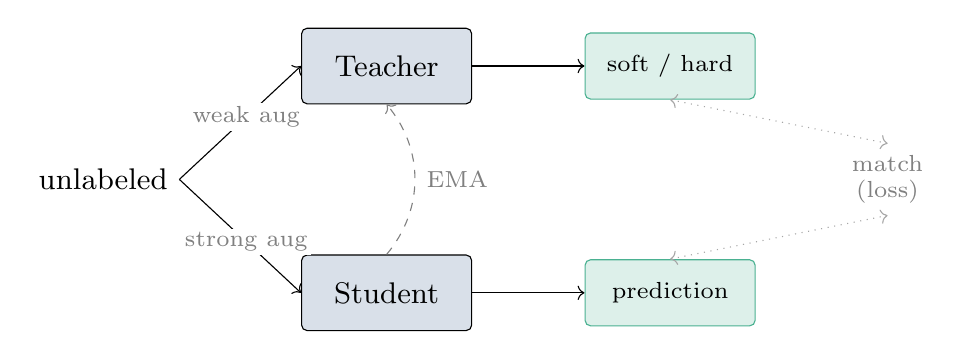
\begin{tikzpicture}[
    scale=1.2, transform shape,
    net/.style={draw=black, fill=PUCBlue!15, rounded corners=2pt, minimum width=1.8cm, minimum height=0.8cm, font=\small},
    aug/.style={font=\scriptsize, gray, fill=white, inner sep=1pt},
    outbox/.style={draw=Accent1!80, fill=Accent1!15, rounded corners=2pt, minimum width=1.8cm, minimum height=0.7cm, font=\scriptsize}
  ]
    % Input
    \node[font=\small] (inp) at (0, 0) {unlabeled};

    % Teacher (arriba)
    \node[net] (teacher) at (3, 1.2) {Teacher};
    \node[outbox] (tout) at (6, 1.2) {soft / hard};

    % Student (abajo)
    \node[net] (student) at (3, -1.2) {Student};
    \node[outbox] (sout) at (6, -1.2) {prediction};

    % Flechas input → nets
    \draw[->] (inp.east) -- node[aug, pos=0.55]{weak aug} (teacher.west);
    \draw[->] (inp.east) -- node[aug, pos=0.55]{strong aug} (student.west);

    % Flechas nets → outs
    \draw[->] (teacher.east) -- (tout.west);
    \draw[->] (student.east) -- (sout.west);

    % EMA (student → teacher)
    \draw[->, dashed, gray] (student.north) to[bend right=40] node[font=\scriptsize, midway, right, gray]{EMA} (teacher.south);

    % Match loss
    \node[font=\scriptsize, align=center, gray] (loss) at (8.3, 0) {match\\(loss)};
    \draw[<->, dotted, gray!70] (tout.south) -- (loss.north);
    \draw[<->, dotted, gray!70] (sout.north) -- (loss.south);
  \end{tikzpicture}
  \caption[Teacher--student framework shared by PL and MT.]{Teacher--student framework shared by Pseudo-Labeling and Mean Teacher. The two methods differ only at the \emph{soft / hard} step: PL binarizes the teacher's output, MT keeps it as a probability map.}
  \label{fig:teacher-student}
\end{figure}

\textbf{Pseudo-Labeling (PL).} A hard pseudo-label $\tilde{y} = \mathbb{1}[p_T \geq 0.5]$ is generated from the teacher's probability map. A confidence mask $\mathcal{M}$ retains only pixels where $p_T \geq \tau$ or $p_T \leq 1 - \tau$, with $\tau = 0.95$ following \citet{ref_fixmatch}. The unsupervised loss is computed only over the confident pixels:
\begin{equation}
\mathcal{L}_U^{\text{PL}} = \frac{1}{|\mathcal{M}|} \sum_{i \in \mathcal{M}} \text{BCE}(p_{S,i}, \tilde{y}_i).
\end{equation}
Pixels outside $\mathcal{M}$ do not contribute to the loss, preventing low-confidence predictions from injecting noise into training.

\textbf{Mean Teacher (MT).} In contrast to PL, no confidence thresholding is applied: the student's predictions are pushed toward the teacher's continuous probability map over all pixels. The unsupervised loss is the mean squared error between the two predictions:
\begin{equation}
\mathcal{L}_U^{\text{MT}} = \text{MSE}(p_S, p_T).
\end{equation}
This formulation provides a soft consistency target, which means every pixel contributes to the loss, including those where the teacher is uncertain. The model keeps information that PL filters out, but at the cost of also learning from noisier predictions.

\section{Unlabeled pool construction and selection policies}
\label{sec:method-pool}

Unlabeled pools are constructed from the same training videos that contain the labeled frames. Given a labeled frame at index $t$, the temporal-neighbor policy selects the lateral frames within the interval $[t-r, t+r]$ that lack a mask. The parameter $r$, called the temporal radius, controls the size of the pool: smaller values produce pools that closely surround the labeled frames, while larger values reach into more distant parts of the swallowing sequence. Six radiuses are evaluated, spanning the time scales of key swallowing events at 30~fps: \citet{ref_kendall2000} report that hyoid elevation to its maximum takes 280--320~ms and that total pharyngeal transit lasts 850--910~ms, so the radiuses range from $r=3$ ($\pm 100$~ms, well within a single sub-event) to $r=20$ ($\pm 667$~ms, approaching the full pharyngeal transit). In addition to these six pools, a larger pool containing all lateral frames from the training videos is included as an upper bound on the available unlabeled data. Table~\ref{tab:pools} reports the resulting pool sizes for UNM.

\begin{table}[!t]
\centering
\footnotesize
\caption[Unlabeled pool sizes per temporal radius in UNM.]{Unlabeled pool sizes for each temporal radius in UNM. Percentages are relative to 74{,}774 UNM lateral training frames. INCA pools were constructed analogously from 31{,}260 lateral training frames.}
\label{tab:pools}
\begin{tabular}{@{}cccc@{}}
\toprule
\textbf{Radius} & \textbf{Frames} & \textbf{\% of training pool} & \textbf{Temporal window} \\
\midrule
$r=3$     & 1{,}257  & 1.7\%   & $\pm$100\,ms \\
$r=5$     & 2{,}066  & 2.8\%   & $\pm$167\,ms \\
$r=7$     & 2{,}849  & 3.8\%   & $\pm$233\,ms \\
$r=10$    & 3{,}937  & 5.3\%   & $\pm$333\,ms \\
$r=15$    & 5{,}590  & 7.5\%   & $\pm$500\,ms \\
$r=20$    & 7{,}081  & 9.5\%   & $\pm$667\,ms \\
All lateral & 74{,}774 & 100\%   & --- \\
\bottomrule
\end{tabular}
\end{table}

To isolate the effect of the selection policy from the effect of pool size, a size-matched random control is constructed for each temporal pool. For every video, the number of unlabeled frames selected at random matches the number selected by the temporal-neighbor policy at the corresponding radius, drawn uniformly from the lateral frames of that video and excluding the labeled frames. This matched design controls for pool size, so that differences in segmentation performance between the two policies at a given radius can be attributed primarily to the temporal distribution of the selected frames rather than to how many were used. The same matching procedure is applied at all six radiuses, yielding six temporal/random pool pairs per dataset.

The combination of these two design choices defines the experimental grid for the pool-composition study. For each of the two SSL methods (PL and MT), the six temporal radiuses are paired with their size-matched random controls, yielding 12 conditions per method, plus the all-lateral pool as an upper bound.

\section{Evaluation protocol}
\label{sec:method-eval}

Segmentation performance is evaluated primarily by the F1 score (equivalent to the Dice coefficient), computed as the per-image average over the test set of each dataset (63 images for UNM, 194 for INCA). Two boundary metrics are additionally reported to capture contour quality beyond region-based overlap: the Average Symmetric Surface Distance (ASSD) and the 95th-percentile Hausdorff Distance (HD95), both expressed in pixels. All three are computed on the $320 \times 320$ grid the models are trained on, against reference masks resampled to the same grid. The two boundary metrics are undefined when a prediction contains no foreground pixels, and those frames are excluded from them. Model selection is performed by validation IoU. To account for training variability, most SSL configurations are run with three random seeds; reference conditions in UNM (the six supervised architectures, PL and MT at $r=10$ temporal, and the supervised and SSL runs at each UNM label fraction) are additionally run with two extra seeds, reflecting the higher between-seed variability observed in UNM's smaller test set. Results are reported as mean $\pm$ standard deviation across seeds. For paired comparisons between conditions, Wilcoxon signed-rank tests are applied to cluster-level mean F1 scores, using patients as clusters in both datasets.

Label-efficiency subsets were constructed differently to account for the structure of each dataset. In UNM, each patient contributes a single long recording, whereas INCA contains shorter recordings and some patients contribute multiple videos. For UNM, fixed nested subsets were sampled within each training video, retaining all 23 training patients while reducing the number of labeled frames from each. For INCA, the subsets contained complete training patients, reducing both the number of labeled frames and the number of patients represented. All subsets were restricted to the original training partition, leaving the validation and test sets unchanged. The same label fraction therefore does not represent the same condition in both datasets.


%% =============================================================================
%%  CHAPTER 4 — Results and Discussion
%% =============================================================================

\chapter{Results and Discussion}
\label{chap:results}

This chapter reports the experimental results. Sections~\ref{sec:results-ssl} and~\ref{sec:results-pool} address the three research questions: how SSL performance changes across labeling regimes (RQ1), and how the unlabeled pool size (RQ2) and the frame selection policy (RQ3) affect results within regimes where SSL helps. Section~\ref{sec:results-archs} then compares SSL configurations against six supervised architectures, and Section~\ref{sec:results-altsettings} examines nnU-Net together with the individual pipeline settings that separate it from the fixed one. Section~\ref{sec:results-boundary} reports analyses beyond F1, Section~\ref{sec:results-uncertainty} the predictive uncertainty of the trained models, and Section~\ref{sec:results-scope} the extent to which the findings depend on the two SSL methods evaluated. Limitations are discussed in Section~\ref{sec:results-limits}.

\section{SSL effect across labeling regimes}
\label{sec:results-ssl}

SSL is expected to help most when the supervised baseline has not yet saturated, that is, when there are too few labeled frames to exploit the model's capacity. UNM, with 218 training frames, provides such a regime. INCA, with 634 training frames, provides a saturated reference; subsampling the labels also enables a controlled reduction to the label-scarce regime.

On UNM, the supervised U-Net++ baseline reached F1~=~0.801~$\pm$~0.014 across five seeds. Both SSL methods improved over this baseline across the full grid of pool conditions: in all 26 SSL configurations (13 pool sizes by two methods), mean F1 matched or exceeded the supervised baseline, and 20 of them showed gains above +0.02. Pseudo-labeling achieved its best result with the smallest temporal pool, reaching F1~=~0.852~$\pm$~0.019 at $r=3$; Mean Teacher reached its best configuration with the all-lateral pool, F1~=~0.860~$\pm$~0.006, which corresponds to a gain of +0.059 over the supervised baseline. Patient-level Wilcoxon signed-rank tests supported the pseudo-labeling improvement across all three seeds ($p=0.016$ in each). For Mean Teacher, two of three seeds showed significant improvements ($p=0.016, 0.016$, and $0.078$), with mean differences remaining positive in all three seeds. These results are consistent with a regime in which the supervised baseline (F1~$<$~0.85) still had room for improvement that additional unlabeled frames could provide.

On INCA with the full training set (634 frames), neither SSL method improved over the supervised baseline. The supervised U-Net++ reached F1~=~0.906~$\pm$~0.003, and the best of the fourteen SSL configurations (pseudo-labeling at $r=20$ temporal) reached F1~=~0.908~$\pm$~0.002, a difference of $+$0.003 that is the same size as the seed-to-seed spread of the baseline itself. To investigate whether this absence of improvement was tied to the higher annotation budget rather than to dataset-specific properties, both methods were re-evaluated on patient-level subsets at 10\%, 25\%, and 50\% of the INCA training set (56, 132, and 283 frames, respectively). At the lowest fraction (56 frames), both methods improved over the supervised baseline: pseudo-labeling reached F1~=~0.854~$\pm$~0.006 ($\Delta=+0.010$) and Mean Teacher reached F1~=~0.865~$\pm$~0.005 ($\Delta=+0.021$). Patient-level Wilcoxon tests supported the Mean Teacher improvement in all three seeds ($p<0.01$ in each); pseudo-labeling showed less consistent seed-level support ($p=0.917, 0.038$, and $0.105$). At 25\% (132 frames) and 50\% (283 frames), the supervised baseline already reached F1~$>$~0.89 and SSL did not yield additional gains.

Detailed label-efficiency values are reported in Table~\ref{tab:label_eff}, and the corresponding trends are shown in Figure~\ref{fig:labeleff}. Taken together, the UNM and INCA results indicate that, in the evaluated conditions, the clearest SSL gains occurred when the supervised baseline remained below approximately F1~=~0.85; once the supervised baseline exceeded about 0.89, SSL did not provide consistent additional gains. This is consistent with the unlabeled frames contributing little beyond what is already captured by a strongly performing labeled set. Table~\ref{tab:ssl_summary} summarizes the supervised baseline and best SSL configurations across all evaluated regimes. Figure~\ref{fig:qualitative} illustrates these contrasting outcomes by comparing supervised and Mean Teacher predictions in two regimes where SSL improves segmentation (UNM and INCA 10\% subset) and one where it does not (INCA full).

\begin{table}[!t]
\centering
\footnotesize
\caption{Supervised baseline and best SSL configurations across evaluated regimes.}
\label{tab:ssl_summary}
\begin{tabular}{@{}lcccc@{}}
\toprule
\textbf{Regime} & \textbf{Supervised} & \textbf{PL best} & \textbf{MT best} & \textbf{$\Delta$ MT} \\
\midrule
UNM full (218 fr.)     & 0.801 $\pm$ 0.014 & 0.852 ($r{=}3$)     & 0.860 (all-lateral) & $+$0.059 \\
INCA full (634 fr.)    & 0.906 $\pm$ 0.003 & 0.908 ($r{=}20$)    & 0.908 ($r{=}3$)     & $+$0.002 \\
INCA 10\% (56 fr.)     & 0.844 $\pm$ 0.006 & 0.854 ($r{=}10$)    & 0.865 ($r{=}10$)    & $+$0.021 \\
INCA 25\% (132 fr.)    & 0.892 $\pm$ 0.002 & 0.887 ($r{=}10$)    & 0.888 ($r{=}10$)    & $-$0.004 \\
INCA 50\% (283 fr.)    & 0.896 $\pm$ 0.004 & 0.894 ($r{=}10$)    & 0.897 ($r{=}10$)    & $+$0.001 \\
\bottomrule
\end{tabular}
\end{table}

\begin{table}[!t]
\centering
\caption[Label-efficiency analysis.]{Label-efficiency analysis: F1 (mean~$\pm$~std across training seeds) on UNM and INCA for the supervised U-Net++ baseline and the two SSL methods at $r{=}10$ temporal. Bold values indicate the best F1 per row.}
\label{tab:label_eff}
\footnotesize
\begin{tabular}{@{}clccc@{}}
\toprule
\textbf{Dataset} & \textbf{Labels} & \textbf{Supervised} & \textbf{PL $r{=}10$} & \textbf{MT $r{=}10$} \\
\midrule
\multirow{4}{*}{UNM}
 & 25\% (66 fr.)  & .807$\pm$.010 & .803$\pm$.023 & \textbf{.816}$\pm$.017 \\
 & 50\% (111 fr.) & \textbf{.823}$\pm$.017 & .819$\pm$.025 & .819$\pm$.011 \\
 & 75\% (174 fr.) & .829$\pm$.017 & .834$\pm$.021 & \textbf{.837}$\pm$.015 \\
 & 100\% (218 fr.) & .801$\pm$.014 & .832$\pm$.012 & \textbf{.850}$\pm$.006 \\
\midrule
\multirow{4}{*}{INCA}
 & 10\% (56 fr.)  & .844$\pm$.006 & .854$\pm$.006 & \textbf{.865}$\pm$.005 \\
 & 25\% (132 fr.) & \textbf{.892}$\pm$.002 & .887$\pm$.003 & .888$\pm$.005 \\
 & 50\% (283 fr.) & .896$\pm$.004 & .894$\pm$.000 & \textbf{.897}$\pm$.003 \\
 & 100\% (634 fr.) & \textbf{.906}$\pm$.003 & .903$\pm$.001 & \textbf{.906}$\pm$.001 \\
\bottomrule
\end{tabular}
\end{table}

\begin{figure}[!htbp]
  \centering
  \includegraphics[width=0.7\textwidth]{fig3_label_efficiency_vertical.pdf}
  \caption[Label-efficiency curves on UNM and INCA.]{F1 on UNM (top) and INCA (bottom) test sets as a function of the labeled data fraction (UNM 100\%~=~218 labeled training frames; INCA 100\%~=~634 labeled training frames). The two panels compare the supervised U-Net++ baseline with pseudo-labeling and Mean Teacher at $r{=}10$ temporal. Shaded bands show $\pm$1 std across training seeds (five for UNM fractions; three for INCA fractions).}
  \label{fig:labeleff}
\end{figure}

\begin{figure*}[!htbp]
  \centering
  \includegraphics[width=\textwidth]{fig5_qualitative_horizontal_annotated.pdf}
  \caption[Qualitative segmentation results.]{Qualitative segmentation results across three label-budget regimes. Columns show UNM, INCA 10\% subset, and INCA full. Rows show the input frame, reference contour (green outline), supervised prediction, and Mean Teacher prediction. In prediction panels, green~=~true positives, red~=~false negatives, and blue~=~false positives. F1 is reported for each prediction; parentheses show $\Delta$ vs the supervised prediction.}
  \label{fig:qualitative}
\end{figure*}

A key practical observation is that segmentation quality remained competitive even under substantial label reduction. In INCA, Mean Teacher with only 10\% of labels (56 frames) reached F1~=~0.865, a 4.1\% reduction from the best supervised result obtained with the full training set (0.906), while also exceeding the same-budget supervised baseline (0.844). In UNM, Mean Teacher with 25\% of labels reached F1~=~0.816, a 1.3\% reduction from the best supervised label-fraction result (0.829), and comparable to the same-budget supervised baseline (0.807).

\clearpage
\section{Effect of pool size and selection policy}
\label{sec:results-pool}

Pool size and selection policy can only affect performance where SSL provides gains, so these analyses focus on UNM and the INCA 10\% subset. INCA with the full training set is reported as a check on that premise. The corresponding pool-size results are in Tables~\ref{tab:ssl_unm_pool} and~\ref{tab:ssl_inca_pool}.

\textbf{Effect of pool size (RQ2).} On UNM, pool size affected the two methods in opposite directions (Figure~\ref{fig:poolsize}). Pseudo-labeling achieved its best F1 with the smallest temporal pool ($r=3$, F1~=~0.852~$\pm$~0.019) and its worst with the largest ($r=20$, F1~=~0.803~$\pm$~0.022), close to the supervised baseline. Mean Teacher showed the inverse pattern, reaching its best result with the all-lateral pool (74{,}774 frames, F1~=~0.860~$\pm$~0.006); among the temporal radiuses, its lowest results occurred at $r=3$, $r=15$ and $r=20$ (F1~$\approx$~0.828), with no monotonic trend across the radiuses. One possible explanation is that the two methods use the teacher's predictions differently. In pseudo-labeling, confident predictions become hard targets, so a prediction that is wrong but confident can reinforce segmentation errors during training. Mean Teacher instead matches the teacher's continuous output, giving a softer training signal that may be less affected by individual errors. On INCA with the full training set, pool size had no discernible effect: across the seven pool sizes and both methods, F1 ranged from 0.902 to 0.908, all within $\pm$0.004 of the supervised baseline. On the INCA 10\% subset (56 frames), pool-size effects were smaller than in UNM but the best pool shifted: pseudo-labeling peaked at $r=10$ (F1~=~0.854~$\pm$~0.006), and its all-lateral configuration performed near the supervised baseline; neither method achieved its best result with the all-lateral pool, suggesting that the best pool choice differs between datasets, even within label-scarce regimes. These observations indicate that pool size should be treated as a hyperparameter to evaluate rather than defaulting to the largest available pool.

\begin{table}[!t]
\centering
\caption[SSL results on UNM at the full label budget.]{SSL results on UNM at the full label budget (218 labeled frames). F1 (mean~$\pm$~std) across training seeds (three for most configurations; five for temporal $r{=}10$). Bold values mark the best per row. Supervised baseline: F1~=~0.801~$\pm$~0.014 (five seeds).}
\label{tab:ssl_unm_pool}
\footnotesize
\resizebox{\textwidth}{!}{%
\begin{tabular}{@{}lccccccc@{}}
\toprule
 & \multicolumn{7}{c}{\textbf{Pool size}} \\
\cmidrule(lr){2-8}
\textbf{Method / Policy} & $r{=}3$ & $r{=}5$ & $r{=}7$ & $r{=}10$ & $r{=}15$ & $r{=}20$ & All lateral \\
\midrule
PL temporal    & \textbf{.852}$\pm$.019 & .831$\pm$.008 & .830$\pm$.019 & .832$\pm$.012 & .840$\pm$.007 & .803$\pm$.022 & .830$\pm$.020 \\
PL random      & .835$\pm$.005 & .826$\pm$.005 & .819$\pm$.027 & .845$\pm$.010 & .846$\pm$.016 & .806$\pm$.042 & $^\star$ \\
\midrule
MT temporal    & .828$\pm$.011 & .837$\pm$.026 & .834$\pm$.025 & .850$\pm$.006 & .828$\pm$.006 & .828$\pm$.019 & \textbf{.860}$\pm$.006 \\
MT random      & .811$\pm$.023 & .836$\pm$.008 & .818$\pm$.030 & .857$\pm$.004 & .830$\pm$.038 & .821$\pm$.026 & $^\star$ \\
\bottomrule
\multicolumn{8}{@{}l}{\footnotesize $^\star$All lateral uses the complete unlabeled pool; no random subsampling applies.}
\end{tabular}%
}
\end{table}

\begin{figure}[!htbp]
  \centering
  \includegraphics[width=0.7\textwidth]{fig2_pool_size_curves_vertical.pdf}
  \caption[Effect of unlabeled pool size in UNM.]{Effect of unlabeled pool size on F1 in UNM at the full label budget (218 labeled frames). The two panels show pseudo-labeling (top) and Mean Teacher (bottom), comparing temporal-neighbor and size-matched random selection across the six temporal radiuses and the all-lateral pool (``All''). Error bars show $\pm$1 std across training seeds (three for most SSL configurations; five for $r{=}10$). Dotted line and gray band: supervised baseline ($0.801 \pm 0.014$, 5 seeds).}
  \label{fig:poolsize}
\end{figure}

\textbf{Effect of frame selection policy (RQ3).} At each pool size, the temporal-neighbor policy was compared against its size-matched random control. In UNM, pseudo-labeling showed mixed differences depending on the radius: temporal selection yielded higher mean F1 than random at small radiuses ($r=3$: 0.852 vs 0.835; $r=7$: 0.830 vs 0.819), but random yielded higher mean F1 than temporal at larger radiuses ($r=10$: 0.832 vs 0.845; $r=15$: 0.840 vs 0.846). However, at the reference radius $r=10$, patient-level Wilcoxon tests did not detect significant differences between policies for either method in any seed (all $p > 0.05$). In the INCA 10\% subset, differences between policies were within 0.001 in most configurations (e.g., $r=10$: 0.854 vs 0.853 for pseudo-labeling), and patient-level Wilcoxon tests also showed no significant differences. At higher INCA label budgets (25\% and 50\%), differences between policies were below 0.001 in most configurations. Across methods, datasets, and pool sizes, neither policy demonstrated a systematic advantage; observed differences were small relative to the effect of pool size itself and to the gap between SSL and supervised training. These results suggest that, within the regimes evaluated here, temporal proximity alone was not a reliable criterion for choosing unlabeled frames.

\begin{table}[!h]
\centering
\caption[SSL results on the INCA 10\% subset.]{SSL results on the INCA 10\% subset (56 labeled frames). F1 (mean~$\pm$~std) across three training seeds. Bold values mark the best per row. Supervised baseline: F1~=~0.844~$\pm$~0.006.}
\label{tab:ssl_inca_pool}
\footnotesize
\begin{tabular}{@{}lcc@{}}
\toprule
\textbf{Pool size} & \textbf{PL temporal} & \textbf{PL random} \\
\midrule
$r{=}3$        & .850$\pm$.003 & .846$\pm$.004 \\
$r{=}10$       & .854$\pm$.006 & .853$\pm$.007 \\
$r{=}20$       & .841$\pm$.015 & .843$\pm$.008 \\
All lateral    & \multicolumn{2}{c}{.844$\pm$.018} \\
\midrule
\textbf{Pool size} & \textbf{MT temporal} & \textbf{MT random} \\
\midrule
$r{=}3$        & .860$\pm$.007 & \textbf{.865}$\pm$.001 \\
$r{=}10$       & \textbf{.865}$\pm$.005 & .857$\pm$.009 \\
$r{=}20$       & .856$\pm$.005 & .862$\pm$.004 \\
All lateral    & \multicolumn{2}{c}{.860$\pm$.004} \\
\bottomrule
\end{tabular}
\end{table}

\FloatBarrier

\section{Comparison with supervised architectures}
\label{sec:results-archs}

To contextualize the SSL results, five supervised architectures were evaluated on UNM alongside the U-Net++ baseline used for SSL: U-Net~\citep{ref_unet}, DeepLabV3+~\citep{ref_deeplabv3plus}, FPN~\citep{ref_fpn}, TransUNet~\citep{ref_transunet}, and a Kim-inspired BiFPN-U-Net(T) adapted from the VFSS literature~\citep{ref_kim2021}. Table~\ref{tab:arch} reports F1, ASSD, and HD95 for each architecture, along with the best SSL configurations under the fixed U-Net++ pipeline and the self-configuring nnU-Net evaluated as a complementary reference.

\begin{table}[H]
\centering
\caption[Architecture baselines and best SSL configurations on UNM.]{Architecture baselines and best SSL configurations on UNM at the full label budget (218 labeled frames). Mean~$\pm$~std across five seeds for the supervised architectures and three for the SSL configurations.}
\label{tab:arch}
\footnotesize
\begin{tabular}{@{}lccc@{}}
\toprule
\textbf{Method} & \textbf{F1} $\uparrow$ & \textbf{ASSD (px)} $\downarrow$ & \textbf{HD95 (px)} $\downarrow$ \\
\midrule
\multicolumn{4}{@{}l}{\emph{Supervised (this pipeline, $320{\times}320$)}} \\
\quad DeepLabV3+      & .776$\pm$.041 & 2.08$\pm$0.23 & 7.07$\pm$0.66  \\
\quad BiFPN-U-Net(T)  & .759$\pm$.012 & 4.86$\pm$1.59 & 12.39$\pm$2.78 \\
\quad U-Net++         & .801$\pm$.014 & 2.41$\pm$0.22 & 9.86$\pm$2.06  \\
\quad FPN             & .799$\pm$.025 & 2.08$\pm$0.20 & 6.55$\pm$0.87  \\
\quad U-Net           & .824$\pm$.032 & 2.09$\pm$0.31 & 8.39$\pm$2.22  \\
\quad TransUNet       & .851$\pm$.011 & 1.92$\pm$0.20 & 8.16$\pm$1.49  \\
\midrule
\multicolumn{4}{@{}l}{\emph{Semi-supervised (U-Net++, this pipeline)}} \\
\quad PL temporal $r{=}3$       & .852$\pm$.019 & 1.76$\pm$0.28 & 6.72$\pm$1.02 \\
\quad MT all lateral            & \textbf{.860}$\pm$.006 & \textbf{1.62}$\pm$0.13 & \textbf{5.68}$\pm$0.37 \\
\midrule
\multicolumn{4}{@{}l}{\emph{Semi-supervised (other backbones, MT size-matched random $r{=}15$)}} \\
\quad DeepLabV3+      & .800$\pm$.014 & 2.24$\pm$0.25 & 8.17$\pm$1.06 \\
\quad BiFPN-U-Net(T)  & .757$\pm$.029 & 5.26$\pm$2.60 & 12.59$\pm$4.24 \\
\quad U-Net++         & .830$\pm$.038 & 1.92$\pm$0.22 & 7.80$\pm$0.93 \\
\quad FPN             & .811$\pm$.028 & 2.24$\pm$0.13 & 7.74$\pm$0.86 \\
\quad U-Net           & .851$\pm$.005 & 1.64$\pm$0.05 & 6.06$\pm$0.74 \\
\quad TransUNet       & .831$\pm$.005 & 2.09$\pm$0.15 & 8.72$\pm$0.88 \\
\bottomrule
\end{tabular}
\end{table}

Performance ranged from BiFPN-U-Net(T) at F1~=~0.759~$\pm$~0.012, which uses VGG16 without ImageNet pretraining, to TransUNet at F1~=~0.851~$\pm$~0.011, the strongest architecture in this pipeline, with U-Net++ at 0.801~$\pm$~0.014. As a control, BiFPN-U-Net(T) was rerun with an ImageNet-pretrained VGG16 encoder, which left F1 at 0.762~$\pm$~0.014 across five seeds. As a complementary control, U-Net++ was trained from scratch, which lowered F1 from 0.801~$\pm$~0.014 to 0.777~$\pm$~0.024. ImageNet pretraining thus gave a modest benefit that varied by architecture, helping U-Net++ but not BiFPN-U-Net(T), and did not by itself account for the differences between architectures. BiFPN-U-Net(T) is also the architecture furthest from the setting it was designed for: the original was trained on 6{,}632 annotated frames, about twenty times the number available here. Adding pretrained weights did not close the gap, so the labeling regime remains a difference this comparison does not isolate.

The best SSL configurations with U-Net++ reached F1 levels comparable to or slightly above the strongest supervised architecture. Pseudo-labeling at $r=3$ temporal achieved F1~=~0.852, and Mean Teacher with the all-lateral pool achieved F1~=~0.860, suggesting that, within the fixed $320 \times 320$ pipeline, unlabeled data can provide gains comparable in magnitude to those obtained by changing the supervised backbone.

To check whether this behavior was specific to U-Net++, one Mean Teacher setting (random pool, $r=15$) was rerun with five additional backbones. U-Net improved from F1~=~0.824 to 0.851~$\pm$~0.005, DeepLabV3+ from 0.776 to 0.800~$\pm$~0.014, and FPN changed only slightly from 0.799 to 0.811~$\pm$~0.028. BiFPN-U-Net(T) did not move, from 0.759 to 0.757~$\pm$~0.029, and TransUNet fell from 0.851 to 0.831~$\pm$~0.005. Under that same setting U-Net++ itself improved from 0.801 to 0.830~$\pm$~0.038 (Table~\ref{tab:arch}), so all six backbones can be compared under one configuration. These additional runs suggest that the use of unlabeled frames is not tied only to U-Net++, though it does not reach every backbone. Four of the six gain between 0.012 and 0.029 F1; BiFPN-U-Net(T) does not move, and TransUNet, the strongest supervised architecture in this pipeline, loses 0.020. The detailed analysis of pool size and selection policy remains based on the U-Net++ pipeline.

\section{nnU-Net and alternative pipeline settings}
\label{sec:results-altsettings}

The architecture comparison kept the training pipeline fixed. As a complementary reference, a self-configuring nnU-Net~\citep{ref_nnunet} was evaluated, since it adapts the training configuration to the dataset; it was trained once per label fraction. Across label fractions, nnU-Net reached F1~=~0.896 (25\%), 0.903 (50\%), 0.908 (75\%), and 0.907 (100\%), already near its maximum at 25\%, above all methods trained under the fixed U-Net++ pipeline. The two pipelines differ substantially in training configuration, in input resolution ($1024 \times 1024$ versus $320 \times 320$), augmentation intensity, training duration (${\sim}$1{,}000 versus ${\sim}$75~epochs), and normalization. nnU-Net rotates by up to $\pm 180^\circ$ and scales within $[0.7, 1.4]$, against $\pm 5^\circ$ and $[0.97, 1.03]$ here. It also normalizes each frame to zero mean and unit variance rather than to the unit interval. All of these are configuration differences rather than differences of learning paradigm, because nnU-Net is itself a supervised system.

Each of those differences was then adopted in the fixed pipeline on its own, with everything else left unchanged, and measured against its own control across three seeds (Table~\ref{tab:alt_settings}). Training at $1024 \times 1024$ changed F1 by $+0.001 \pm 0.036$, with both arms trained on six images per step, since the batch used elsewhere does not fit at the higher resolution. The moderate nnU-Net augmentation profile changed it by $-0.003 \pm 0.038$, and the full profile by $-0.017 \pm 0.014$, the only one of the four in which all three seeds moved in the same direction. Per-frame z-score normalization gave $-0.012 \pm 0.064$. Training duration was not adopted in the same way, since the shorter schedule was never imposed; every run of the fixed pipeline was allowed 2{,}000 epochs and stopped when validation performance stopped improving. No setting produced a measurable improvement, and the only consistent change was a decrease under the full augmentation profile, so none of these choices accounts on its own for the difference.

The three alternative intensity treatments were examined in the same way, since the acquisition is grainy and the bony boundaries are often faint (Table~\ref{tab:alt_settings}). Soft CLAHE changed F1 by $-0.015 \pm 0.015$ and global histogram equalization by $-0.016 \pm 0.061$, neither of them an improvement, while non-local means denoising lowered it by $0.096 \pm 0.060$, with all three seeds falling. The frames are therefore left at their acquired intensities.

\begin{table}[!htbp]
\centering
\caption{Change in F1 when each alternative setting is adopted in the fixed pipeline.}
\label{tab:alt_settings}
\footnotesize
\begin{tabular}{@{}lcc@{}}
\toprule
\textbf{Setting} & \textbf{$\Delta$ F1} & \textbf{Seeds improving} \\
\midrule
\multicolumn{3}{@{}l}{\emph{Adopted from nnU-Net}} \\
\quad Input resolution $1024{\times}1024$ & $+0.001 \pm 0.036$ & 2 of 3 \\
\quad Augmentation, nnU-Net moderate      & $-0.003 \pm 0.038$ & 2 of 3 \\
\quad Augmentation, nnU-Net full          & $-0.017 \pm 0.014$ & 0 of 3 \\
\quad Per-frame z-score normalization     & $-0.012 \pm 0.064$ & 1 of 3 \\
\midrule
\multicolumn{3}{@{}l}{\emph{Alternative intensity treatments}} \\
\quad Soft CLAHE                          & $-0.015 \pm 0.015$ & 1 of 3 \\
\quad Global histogram equalization       & $-0.016 \pm 0.061$ & 1 of 3 \\
\quad Non-local means denoising           & $-0.096 \pm 0.060$ & 0 of 3 \\
\bottomrule
\end{tabular}
\end{table}

The Mean Teacher comparison was run on nnU-Net as well, to test whether the same effect appears in a pipeline it does not share. Under a matched 150-epoch schedule at 25\% labels, Mean Teacher reached F1~=~0.868, compared with 0.863 for a supervised nnU-Net baseline trained under the same schedule. This comparison is separate from the main nnU-Net results above, which used a longer schedule. The small difference is consistent with the saturation pattern seen earlier: when the supervised baseline is already strong, SSL leaves little room to improve. These results suggest that SSL and pipeline optimization are complementary directions rather than direct substitutes: SSL improves performance by using unlabeled frames without changing the backbone, while self-configuring pipelines like nnU-Net adapt their training configuration to the dataset.

\section{Complementary analyses}
\label{sec:results-boundary}

\textbf{Boundary metrics.} Across the SSL configurations, ASSD and HD95 largely tracked F1. The exception was the reduced-label INCA setting. With the largest pseudo-labeling pools, F1 stayed at the supervised level (0.841--0.844 versus 0.844), while HD95 rose to 29.0~$\pm$~13.1~px at $r{=}20$ and 26.5~$\pm$~22.2~px with the all-lateral pool, against 14.0~$\pm$~7.1~px for the supervised baseline. Mean Teacher was not affected at any pool size. F1 alone can therefore miss this kind of contour degradation.

\textbf{Per-vertebra agreement and the C2--C4 scalar.} Semi-supervised training did not benefit the three vertebrae equally. Each prediction was split into C2, C3 and C4 using the connected components of the reference mask, ordered supero-inferiorly. On UNM the improvement was largest where the supervised model was weakest: with the all-lateral pool, C4 gained 0.090 Dice and C2 only 0.049 (Table~\ref{tab:pervertebra}, Figure~\ref{fig:c4zoom}). Frames in which a reference vertebra received no predicted pixels at all fell from 7.6\% to 1.3\% under Mean Teacher with the temporal pool at $r{=}10$. On INCA at the full label budget the values were high and uniform for Mean Teacher at $r{=}15$ (C2: 0.914, C3: 0.933, C4: 0.927), as expected where the supervised baseline is already saturated.

The C2--C4 anatomical scalar~\citep{ref_molfenter} measures the distance between a corner of C2 and a corner of C4, so C4 is one of the two vertebrae it depends on. On UNM, however, that gain did not carry into the scalar itself: its median error dropped by only 15\%, from 9.3 to 7.9~px. The upper tail barely moved, with the 90th percentile falling from 42.1 to 40.8~px and the largest error from 90.0 to 89.7~px. The reason is the rule that locates those corners, which splits the mask at the gaps between vertebrae. Applying that rule to the reference masks, where the segmentation is correct by construction, still leaves a median error of 6.9~px (Figure~\ref{fig:c2c4floor}). That floor accounts for 87\% of the Mean Teacher error and 74\% of the supervised one, so better masks cannot move the scalar much further. Further gains in the scalar would therefore have to come from the rule itself, or from predicting the corners directly as in \citet{ref_zhang2021}, rather than from better masks.

\begin{table}[!t]
\centering
\caption[Per-vertebra agreement and boundary error on UNM.]{Per-vertebra Dice, frequency of undetected vertebrae, and boundary error on UNM at the full label budget (218 labeled frames). Mean~$\pm$~std across training seeds (five for the supervised baseline and for $r{=}10$; three otherwise). \emph{Missing} is the percentage of test frames in which at least one reference vertebra received no predicted pixels. Bold marks the best value per column.}
\label{tab:pervertebra}
\footnotesize
\resizebox{\textwidth}{!}{%
\begin{tabular}{@{}lcccccc@{}}
\toprule
\textbf{Method} & \textbf{C2} & \textbf{C3} & \textbf{C4} & \textbf{Missing (\%)} $\downarrow$ & \textbf{ASSD (px)} $\downarrow$ & \textbf{HD95 (px)} $\downarrow$ \\
\midrule
Supervised           & .811$\pm$.014 & .834$\pm$.036 & .759$\pm$.018 & 7.6 & 2.41$\pm$0.22 & 9.86$\pm$2.06 \\
\midrule
PL temporal $r{=}3$  & .849$\pm$.030 & .886$\pm$.015 & .846$\pm$.019 & 3.2 & 1.76$\pm$0.28 & 6.72$\pm$1.02 \\
MT temporal $r{=}10$ & \textbf{.863}$\pm$.011 & .878$\pm$.006 & .839$\pm$.012 & \textbf{1.3} & 1.86$\pm$0.32 & 7.66$\pm$1.94 \\
MT all lateral       & .860$\pm$.011 & \textbf{.896}$\pm$.011 & \textbf{.849}$\pm$.020 & 2.1 & \textbf{1.62}$\pm$0.13 & \textbf{5.68}$\pm$0.37 \\
\bottomrule
\end{tabular}%
}
\end{table}

\begin{figure}[!htbp]
  \centering
  \includegraphics[width=0.92\textwidth]{fig_c4_zoom_v2.pdf}
  \caption[Segmentation of C4 in three test frames.]{Segmentation of C4 in three UNM test frames, for the supervised baseline (top) and Mean Teacher with the all-lateral pool (bottom). Green~=~true positives, red~=~false negatives, blue~=~false positives, restricted to the region assigned to C4. The supervised model recovers only part of the vertebra in these frames.}
  \label{fig:c4zoom}
\end{figure}

\begin{figure}[!htbp]
  \centering
  \includegraphics[width=0.9\textwidth]{fig_c2c4_floor.pdf}
  \caption[C2--C4 scalar error by the input given to the post-processing rule.]{C2--C4
  scalar error on the UNM test set, grouped by what the post-processing rule received as
  input: the reference masks (63 frames), the Mean Teacher predictions (63 frames
  $\times$ 3 seeds) and the supervised predictions (63 frames $\times$ 5 seeds). The rule needs the mask to split into three components, and each panel gives the number of predictions for which that was possible. Boxes
  span the interquartile range, whiskers the 10th to 90th percentiles, and the label is
  the median.}
  \label{fig:c2c4floor}
\end{figure}

\textbf{Placement of a region of interest for a downstream task.} Losing a vertebra matters beyond the Dice score. \citet{ref_lee2020} place a dynamic region of interest for airway-invasion detection relative to the centroid of the segmented cervical column, extended anteriorly because the bolus passes in front of the spine. That window has a fixed size, so the segmentation does not resize it, only moves it. The mask therefore contributes only a position, and the error it introduces is a distance.

On the UNM test set, after discarding stray components smaller than 200~px, that centroid fell 6.09~$\pm$~0.53~px from the reference for the supervised baseline and 4.62~$\pm$~0.57~px for Mean Teacher with the all-lateral pool (mean~$\pm$~SD across seeds, 320$\times$320 grid). Mean Teacher was closer in 44 of the 63 frames ($p<0.001$, Wilcoxon).

Some predictions could not be anchored. Nine of the 315 supervised predictions (63 frames $\times$ 5 seeds), spread over four frames, kept no component above the 200~px threshold, so no centroid could be computed and those nine are absent from the 6.09~px above; Mean Teacher produced a usable mask in every frame. Figure~\ref{fig:roilee} illustrates one such case, where the missing C4 pulls the anchor upwards and the whole window follows. This measures where the window lands, not whether invasion is detected, because neither dataset annotates the bolus. The predicted mask locates the column well enough to anchor the window, and a better mask places it closer.

\begin{figure}[!htbp]
  \centering
  \includegraphics[width=0.95\textwidth]{fig_roi_lee.pdf}
  \caption[Placement of a dynamic region of interest.]{Placement of a dynamic region of interest on one UNM test frame. Yellow is the prediction, blue dashed the reference contour, \texttt{+} the reference centroid and \texttt{x} the predicted one. The two rectangles are identical in size and follow the proportions of \citet{ref_lee2020}, $0.7R$ anterior and $0.3R$ posterior; the grey one is anchored on the reference centroid, the solid one on the prediction. The scale $R$ is illustrative.}
  \label{fig:roilee}
\end{figure}

\section{Predictive uncertainty}
\label{sec:results-uncertainty}

Uncertainty is measured per pixel as the binary entropy of the predicted probability, $H(p) = -(p \ln p + (1-p)\ln(1-p))$, computed on the saved test-set probability maps; its maximum is $\ln 2 = 0.693$. Values are reported inside a band around the reference contour, obtained as the morphological dilation of the mask minus its erosion, five iterations each with 4-connectivity, so every pixel in it lies within 5~px of the contour. They are averaged over band pixels per frame, then over frames per seed, and reported as mean~$\pm$~SD across seeds.

\textbf{Location of the uncertainty.} Uncertainty was confined to the vertebral region. Band entropy averages 0.049 on UNM, against 0.029 inside the vertebrae, 0.022 in the gaps between them and 0.0005 in the background (Figure~\ref{fig:uncertainty}); on the INCA 10\% subset the band value is 0.054. Narrowing the band to $\pm$3~px or widening it to $\pm$10~px leaves the ordering unchanged. The errors sit in the same band. It covers 2.6\% of the image on UNM and 3.4\% on the INCA subset, and in both it contains between 80\% and 90\% of the pixels where prediction and reference disagree.

\textbf{Effect of semi-supervised training and pool size.} Semi-supervised training did not make the models more certain. Band entropy was 0.049 for the supervised baseline and 0.048 for Mean Teacher on UNM, and rose from 0.054 to 0.067 on INCA. What changed was where the uncertainty sat: on UNM it fell from 0.029 to 0.020 inside the vertebrae and rose from 0.022 to 0.062 in the gaps between them. It also tracked errors more closely: the Spearman correlation between band entropy and per-frame Dice went from $-$0.25 to $-$0.51 on UNM and stayed near $-$0.5 on INCA under both regimes. Part of the UNM correlation follows vertebral area.

Pool size does not change it either (Figure~\ref{fig:uncpool}). From 1{,}257 to 74{,}774 unlabeled frames, band entropy stays between 0.041 and 0.049, with no monotonic trend (Spearman $\rho = -0.04$, $p = 0.94$). The spread across pools, 0.008, is smaller than the seed-to-seed standard deviation of the supervised baseline, 0.012, and every pool falls within one standard deviation of it. Changing the seed moves entropy more than increasing the pool sixtyfold.

\begin{figure}[!htbp]
  \centering
  \includegraphics[width=0.88\textwidth]{fig_uncertainty_v2.pdf}
  \caption[Predictive uncertainty on three UNM test frames.]{Binary entropy in three UNM test frames, cropped around the vertebrae, for the supervised baseline (top) and Mean Teacher with the all-lateral pool (bottom). The dashed blue line is the reference contour; all panels share the same scale, 0 to $\ln 2$. Entropy is near zero away from the vertebrae and traces their outlines.}
  \label{fig:uncertainty}
\end{figure}

\begin{figure}[!htbp]
  \centering
  \includegraphics[width=0.85\textwidth]{fig_uncertainty_vs_pool.pdf}
  \caption[Band entropy against unlabeled pool size on UNM.]{Band entropy on the UNM test set for Mean Teacher trained with each unlabeled pool: the six temporal radiuses and the all-lateral pool, spanning 1{,}257 to 74{,}774 frames. Error bars and the shaded band are $\pm$1 standard deviation across seeds.}
  \label{fig:uncpool}
\end{figure}

\textbf{Use of uncertainty for frame selection.} Whether that is enough to guide frame selection depends on the dataset. Taking the 20\% most uncertain frames isolated poorer predictions on INCA: Dice 0.78, against [0.82, 0.86] for a random subset of the same size. UNM points the same way, 0.77 against a random mean of 0.80, but its random interval spans [0.70, 0.88] and the difference is not resolvable; with 63 test frames from seven patients that interval is 4.5 times wider than on INCA. The UNM result is inconclusive rather than negative.

Uncertainty was therefore not used to filter the unlabeled pool in the main experiments, although four ways of building it were compared directly at $r=10$ (Table~\ref{tab:pool_policy}). Both entropy-selected pools scored above the temporal one in all three seeds, by $0.037$ and $0.030$, while the size-matched random pool did not separate from it ($+0.003 \pm 0.039$). The pool built from the most uncertain frames and the one built from the least differed by $0.007 \pm 0.037$ across three seeds, so it made no measurable difference which end of the entropy ranking the pool came from. The boundary metrics did not separate the policies either: none of the three differences against the temporal pool exceeded its own spread across seeds.

\begin{table}[!htbp]
\centering
\caption[Change in F1 by unlabeled pool selection policy.]{Change in F1 when the unlabeled pool at $r=10$ is built by a different policy, relative to the temporal-neighbor pool. Mean Teacher on UNM, three seeds each; all four pools contain 3{,}937 frames.}
\label{tab:pool_policy}
\footnotesize
\begin{tabular}{@{}lcc@{}}
\toprule
\textbf{Pool selection policy} & \textbf{$\Delta$ F1} & \textbf{Seeds improving} \\
\midrule
Most uncertain frames   & $+0.037 \pm 0.030$ & 3 of 3 \\
Least uncertain frames  & $+0.030 \pm 0.013$ & 3 of 3 \\
Random, size-matched    & $+0.003 \pm 0.039$ & 2 of 3 \\
\bottomrule
\end{tabular}
\end{table}


\section{Generality across SSL methods}
\label{sec:results-scope}

Pseudo-labeling and Mean Teacher were selected as representatives of two SSL families used in segmentation: self-training and consistency regularization. More recent methods such as FixMatch~\citep{ref_fixmatch} and cross-pseudo supervision~\citep{ref_cps} are refinements within these same families, introducing confidence thresholding or dual-network supervision rather than constituting new families. The two families evaluated here already behave alike. Across the eight labeling regimes of Table~\ref{tab:label_eff}, in which the unlabeled pool is held at $r=10$ for both methods, the effect of SSL over the supervised baseline ranges from $-0.005$ to $+0.049$, while the two methods differ from each other by at most 0.018 in any single regime and by less than 0.005 in five of the eight. The labeling regime therefore accounts for far more of the effect than the choice of method within these families.

\section{Limitations}
\label{sec:results-limits}

This study has limitations that are worth noting. First, the two SSL methods evaluated represent two common families for segmentation (self-training and consistency regularization); whether the regime-dependent benefit extends to other SSL approaches, such as adversarial perturbation or contrastive pretraining, remains to be examined. Second, the main SSL analysis was conducted with a single backbone (U-Net++ with EfficientNet-B3 at $320 \times 320$ resolution), so that changes in performance could be attributed to the SSL setting rather than to architectural differences. Mean Teacher was also run with U-Net, FPN, DeepLabV3+, TransUNet, and BiFPN-U-Net(T), and with nnU-Net at its higher resolution, but only in one configuration each. The pool-size and selection-policy trends should therefore be read as results of the U-Net++ pipeline rather than as general claims across architectures and resolutions. Third, although the two datasets originate from different institutions, both consist of lateral VFSS recordings of the cervical region; the transferability of these findings to other fluoroscopic views or anatomical structures lies outside the scope of this work.

Fourth, the UNM test set contains seven patients, which constrains the statistical power of patient-level tests; with only seven samples, exact Wilcoxon $p$-values can take only a limited set of discrete values. For this reason, UNM $p$-values should be interpreted alongside effect sizes and seed-level consistency. Fifth, external reproducibility of the INCA results is constrained by the institutional data-sharing agreement governing the dataset; the UNM subset, in contrast, is derived from a publicly available source. Sixth, the pseudo-labeling condition combines FixMatch-style confidence thresholding with an EMA teacher and should therefore be interpreted as a pseudo-labeling baseline rather than a direct reproduction of FixMatch. Finally, the reference masks carry inherent variability. Agreement with the speech-language pathologist ($0.854 \pm 0.062$ in UNM and $0.806 \pm 0.082$ in INCA) should be interpreted as consistency with the adopted annotation criteria, since the specialist also contributed clinical input during protocol definition, rather than as fully independent external validation. Dice scores should therefore be interpreted with respect to the adopted reference annotations, not as absolute measures of segmentation quality.

Overall, this work should be interpreted as a feasibility study of semi-supervised learning for cervical vertebra segmentation in VFSS under limited annotation regimes. The reported Dice/F1 scores quantify agreement with the adopted reference annotations, which were produced by trained annotators following an expert-informed annotation procedure. They should therefore not be interpreted as final clinical validation. Clinical deployment would require further validation with additional domain experts and prospective evaluation in the target clinical workflow.


%% =============================================================================
%%  CHAPTER 5 — Conclusion
%% =============================================================================

\chapter{Conclusion}
\label{chap:conclusion}

This work presented a systematic evaluation of semi-supervised learning for cervical vertebra segmentation in VFSS across two institutional datasets (UNM and INCA), using pseudo-labeling and Mean Teacher. The main finding is that SSL achieved F1 comparable to or above supervised training at matched label budgets, with Mean Teacher preserving segmentation quality under aggressive label reduction (only 4.1\% F1 loss in INCA with 10\% labels, and 1.3\% F1 loss in UNM with 25\% labels compared to the best supervised label-fraction result). The largest improvements occurred where the supervised baseline had not yet saturated: in UNM, Mean Teacher improved F1 by up to $+$0.059 over the supervised full-label baseline ($+$0.031 vs the best supervised label-fraction result), while in INCA with only 56 labeled frames (10\% labels), Mean Teacher improved F1 from 0.844 to 0.865 over supervised training at the same budget. At 25\% labels and above in INCA, SSL provided no meaningful improvement, consistent with supervised saturation.

Two additional findings characterize how SSL operates in this setting. First, the optimal unlabeled pool size was method-dependent, with the best-performing pseudo-labeling and Mean Teacher configurations in UNM occurring at opposite extremes of the pool-size range; using all available unlabeled frames did not consistently yield the best results. Second, temporal-neighbor frame selection showed no systematic advantage over size-matched random selection, suggesting that temporal proximity alone was not a reliable criterion for selecting unlabeled frames in this setting.

The practical implication is that, in low-label, unsaturated settings, SSL can improve segmentation performance by leveraging unlabeled frames naturally present in VFSS video. Future work should test whether these patterns hold for structurally different SSL paradigms, such as adversarial perturbation or contrastive pretraining. Beyond cervical vertebra segmentation, the experimental design and findings of this study serve as a basis for future applications of classical SSL to other VFSS segmentation tasks, such as hyoid bone, bolus, residue, and airway segmentation, and to other fluoroscopic imaging domains where labeled data are scarce but unlabeled video is abundant.


%% =============================================================================
%%  CHAPTER 6 — Bibliography
%% =============================================================================

\renewcommand{\bibsection}{}
\chapter{Bibliography}
\label{chap:bibliography}

  \arial
  \bibliography{tesis_sqa}
  \normalfont

%% =============================================================================
%%  APPENDIX A — Consolidated Annotation and Quality-Control Procedure
%% =============================================================================

\appendix

\chapter{Reference Annotation and Quality-Control Procedure}
\label{app:annotation}

This appendix summarizes the reference annotation and quality-control procedure used to generate the reference masks. The description follows reporting principles from the CLAIM 2024 checklist~\citep{ref_tejani2024claim}, especially those related to reference-standard definition, annotation source, test-set annotation, and inter-annotator variability. It also describes how annotation quality was reviewed. The appendix is intended as methodological documentation, not as a clinical annotation protocol.

\section*{A.1 Reference Mask Generation}

The annotation target was the visible cervical vertebral region in lateral VFSS frames, with C2, C3, and C4 as the primary structures of interest. Adjacent vertebrae could also be included in the mask when clearly visible and not truncated by the frame border, but the anatomical reference for downstream measurements remained the C2--C4 region.

Frames were considered annotatable when the cervical vertebral region was sufficiently discernible in the lateral view. Frames were excluded when the cervical vertebrae could not be reliably identified, either because they fell outside the imaging window or because of motion blur, low contrast, view transitions, or other image-quality issues.

Annotations were produced in ImageJ using the freehand selection tool, with local corrections made when necessary. Each mask was exported as a binary image (foreground~=~vertebral region, background~=~0). A vertebra was included when its outline was judged visible by the annotator. When a selected frame was difficult to interpret because of blur or low contrast, annotators could inspect the corresponding video to examine the surrounding frames before completing the mask.

\section*{A.2 Use and Limitations of the Reference Standard}

For the C2--C4 anatomical scalar~\citep{ref_molfenter} used in this domain, the relevant clinical measurement is based on reference points rather than full vertebral masks. Pixel-level segmentation masks were nevertheless adopted as the reference standard here, since downstream tasks in VFSS analysis also include region-based tasks such as dynamic region-of-interest definition~\citep{ref_lee2020} and shape-dependent analyses for which point coordinates are insufficient~\citep{ref_fujinaka}, which require the full spatial extent of the vertebral region.

Recognized limitations of the adopted reference standard include: (i)~annotations were produced by trained annotators rather than clinical specialists delineating every frame; (ii)~cervical vertebral boundaries in VFSS can be ambiguous because of low contrast, overlapping soft tissue, osteophytes, and overlapping bony shadows; and (iii)~partially visible adjacent vertebrae and faint vertebral edges can be difficult to annotate consistently. The upper portion of C2 was a recurrent source of boundary differences during quality review. These issues likely contributed to the inter-annotator variability reported in Section~A.5.

\section*{A.3 Annotation Sources and Clinical Guidance}

\textbf{UNM.} Annotations for the UNM subset were produced by a single graduate student affiliated with the research group, without formal clinical training. The annotation criteria were developed with input from a speech-language pathologist, who provided clinical guidance on vertebral identification, discussed example frames with the team, and remained available for annotation questions during the process.

\textbf{INCA.} Annotations for the INCA dataset were produced by five graduate students affiliated with the research group, also without formal clinical training. They followed the same annotation criteria used for the UNM subset. Clinical guidance was provided by the same speech-language pathologist at the partner institution, with clinical experience in oncology dysphagia, including discussion of example frames and recurring sources of ambiguity. All five annotators received the same general instructions.

\section*{A.4 Test-Set Annotation}

Test-set annotations followed the same procedure, tool, and criteria as the training and validation annotations. Therefore, model performance was evaluated against the same type of reference annotation used throughout the dataset.

\section*{A.5 Annotation Agreement and Variability}

The consistency of the reference annotations was assessed in two ways:

\textbf{Within-team agreement (INCA).} Each of the 898 doubly annotated INCA frames was evaluated by computing the Dice agreement between the two independent masks produced by graduate-student annotators. The mean pairwise Dice agreement was $0.874 \pm 0.070$ (median~0.899).

\textbf{Agreement with the clinical specialist.} To assess consistency with the adopted annotation criteria, the speech-language pathologist who provided clinical input on annotation criteria and annotation questions re-segmented 20 UNM frames and 20 INCA frames without seeing the original masks. These values reflect agreement with the adopted criteria rather than independent external validation. The resulting Dice agreements were $0.854 \pm 0.062$ for UNM and $0.806 \pm 0.082$ for INCA.

\textbf{Discrepancy handling.} For the experiments reported here, one annotation per doubly annotated INCA frame was selected at random as the reference mask before the disagreement review was completed. The within-team agreement reported above suggests that paired annotations were generally similar, but random selection remains a simplification. After model training, frames with substantial inter-annotator disagreement were flagged for re-annotation as part of the dataset quality review. These revised annotations were not incorporated into the experiments reported here. Future curated versions of the dataset should resolve discrepant frames through consensus review with the annotation team or review by the clinical specialist, rather than random selection.

\section*{A.6 Annotation Issues Identified During Quality Review}

During dataset quality review, masks flagged as problematic were grouped into recurring issue types. These categories were used to guide re-annotation and were not part of the original mask labels:

\begin{itemize}
  \item \textbf{(A) Missing vertebra:} a visible vertebra was not segmented.
  \item \textbf{(B) Extra vertebra:} a vertebra was segmented although it was truncated or its outline could not be reliably identified.
  \item \textbf{(C) Overextended vertebra:} part of a vertebra, often the upper or anterior portion of C2, was segmented beyond its visible anatomical boundary.
  \item \textbf{(D) Boundary error:} the mask boundary extended into regions that did not appear to correspond to vertebral bone.
\end{itemize}

Each flagged mask was recorded with its video and frame identifier and a short reason written by the reviewer, in free text. The categories above group those reasons. Figure~\ref{fig:annotissues} shows one example of each type.


\begin{figure}[!htbp]
  \centering
  \includegraphics[width=\textwidth]{fig_annotation_issues.pdf}
  \caption[Examples of the annotation issue types.]{One INCA frame per issue type, each annotated twice. Left: the raw frame; right: both annotations, with an arrow at the point of disagreement. (A)~and~(B) look alike: in both, one annotation has an extra vertebra. The difference is one of judgement: in~(A) the vertebra is visible and the second annotator missed it, while in~(B) its outline is too faint to trace and it should have been left out.}
  \label{fig:annotissues}
\end{figure}

\end{document}
